\documentclass[0pt, a4paper]{article} 
\usepackage[margin=1.00in, a4paper]{geometry}

\setlength{\parindent}{15pt}					% Default is 15pt
\setlength{\parskip}{4pt plus1pt minus0.5pt}	% To set spacing after paragraphs
\usepackage{graphicx}
\usepackage{indentfirst}
\usepackage{amsmath, amssymb, amsfonts}            
\usepackage{color, linegoal}
\usepackage{amsthm, array}
\usepackage[framemethod=tikz]{mdframed}
\usepackage{parskip}
\usepackage{xcolor}
\usepackage{physics}

%%%%%%%%%%%%%%

%\usepackage[
%backend=biber,
%style=authoryear-icomp,
%sortlocale=de_DE,
%natbib=true,
%url=false, 
%doi=true,
%eprint=false
%]{biblatex}
%
%\addbibresource{biblatex-examples.bib}

\usepackage[]{hyperref}
\hypersetup{
	colorlinks=true,
}

\usepackage[noabbrev, capitalize]{cleveref}
\newcommand{\Lagr}{\mathcal{L}}
%%%%%%%%%%%%%%

\title{%
  Notes from Cesaltina\\
  \large 1302 Calculus II}
\date{2018/2019}
\author{Tiago Louro Alves}

\begin{document}

\maketitle
\pagenumbering{arabic}
\thispagestyle{empty}
\newpage

{\small\tableofcontents}

\clearpage

\addcontentsline{toc}{section}{1 Limits and Contituity}
\section*{1 Limits and Continuity}

\addcontentsline{toc}{subsection}{1.1 Notion of function}
\subsection*{1.1 Notion of function}

A function $f$ is the set of ordered pairs $(x,y)$, with $x\in X$ and $y\in Y$, such that there are no two ordered pairs with the same first element. The set of all the elements of $x$ is the domain of $f$, and the set of all elements of $y$ is the codomain of $f$. By $y=f(x)$, we mean that $y$ is determined in a unique way, once one knows $x$. The input of a function is $x$ an $y$ is its output.

\addcontentsline{toc}{subsection}{1.2 $\mathbb{R}^n$ Space}
\subsection*{1.2 $\mathbb{R}^n$ Space}

Properties of the norm of a vector:
\begin{enumerate}
	\item $\norm{\textbf{x}}>0$ if $\textbf{x}\neq0$, and $\norm{\textbf{x}}=0$ if $\textbf{x}=0$; 
	\item $\norm{\lambda \textbf{x}} = \abs{\lambda}\norm{\textbf{x}}$, $\lambda$ being a real number;
	\item $\norm{\lambda \textbf{x}} = \norm{\textbf{x}}+\norm{\textbf{y}}$.
\end{enumerate}	

Distance is defined in a set of points $S$, when each ordered pair $d(\textbf{s}_1, \textbf{s}_2) \in S \times S$ is associated with a non-negative real number $d(\textbf{s}_1, \textbf{s}_2)$ with the following properties:
\begin{enumerate}
	\item $d(\textbf{s}_1, \textbf{s}_2)>0$ if $\textbf{s}_1 \neq \textbf{s}_2$, and $d(\textbf{s}_1, \textbf{s}_2)$=0 if $\textbf{s}_1= \textbf{s}_2$;
	\item $d(\textbf{s}_1, \textbf{s}_2)=d(\textbf{s}_2, \textbf{s}_1)$;
	\item $d(\textbf{s}_1, \textbf{s}_3) \leq d(\textbf{s}_1, \textbf{s}_2)+ (\textbf{s}_2, \textbf{s}_3)$.
\end{enumerate}	

It is interesting to note that all normed vector spaces can be transformed in a metric space. For that to happen, one needs only to define the distance between two vectors, $\textbf{x}$ and $\textbf{y}$, by the equality $d(\textbf{x}, \textbf{y}) = \norm{\textbf{x}-\textbf{y}}$. On the other hand, it is not always possible to transform a metric space into a normed vector space.

\addcontentsline{toc}{subsection}{1.3 Functions of $\mathbb{R}^n$ in $\mathbb{R}^m$}
\subsection*{1.3 Functions of $\mathbb{R}^n$ in $\mathbb{R}^m$}

If $m=1$ and $n=1$, that is, if $f:D \subseteq \mathbb{R} \rightarrow \mathbb{R}$, the scalar function is a \textit{real function of real variable}. If $m=1$ and $n>1$, that is, if $f:D \subseteq \mathbb{R}^n \rightarrow \mathbb{R}$, the scalar function is a \textit{real function of real variables}.

\addcontentsline{toc}{subsection}{1.4 Limit of a function}
\subsection*{1.4 Limit of a function}

There is a parallelism between the concept of a limit of a succession and the notion of limit of a function.

A succession of real numbers is a very special function: it is a function that associates a real number $u_n$ to each natural number $n$. By other words, the domain of a succession is $\mathbb{N}=\{1,2,3,\dots, n, \dots\}$. A succession of images $u_1, u_2, \dots, u_n, \dots$ defines an infinite succession of real numbers. The interesting part is that each element of the succession indicates what is the order of that element in the succession in the sequence: $u_1$ is the first term of the succession, $u_2$ is the second, and so on.

The main objective is to check whether the terms of the succession converge or not to a determined finite value, as $n$ increases indefinitely. When do we say that a succession $u_n$, converges to $u$? Or, by other words, that the succession $u_n$ tends for $u$ when $n$ tends to infinity? A succession $u_n$ is said to converge to $u$, if it is possible to approximate to $u$ as much as we want. That is, for any small value, $\delta>0$, that we can think of, from certain point on, all elements of the succession are less than $\delta$ away from $u$.

Formally, a succession $u_n$ is said to converge to $u$ (or that $\lim_{n \rightarrow \inf} u_n =u$), if $\forall \delta>0, \exists N \in \mathbb{N}:n\geq N \Rightarrow \abs{u_n-u}<\delta$. 

Topology definitions:
\begin{itemize}
	\item Open ball of center $\textbf{c}$ and radius $r$ | $B_r(\textbf{c})=\textbf{x}:\{\norm{\textbf{x}-\textbf{c}}\}<r$;
	\item Closed ball of center $\textbf{c}$ and radius $r$ | $B_r(\textbf{c})=\textbf{x}:\{\norm{\textbf{x}-\textbf{c}}\}\leq r$;
	\item Open set if $S = \text{int }S$;
	\item Closed set is the reunion of the set with its frontier | $\overline{S}=S \cup \text{bd }S$;
	\item Closed set if $S = \overline{S}$;
	\item Disconnected set if $\exists A,B: S=A\cap B \wedge \overline{A}\cap B=\emptyset\wedge A \cap \overline{B}= \emptyset$;
	\item A set is connected if it is not disconnected;
\end{itemize}	

The difference relative to successions is that, when studying limits, instead of a succession of numbers $(u_1, u_2, \dots)$ we have a continuum of points $\textbf{f(x)}$ and the limit of the function is taken as $\textbf{x}$ gets close to $\textbf{a}$. 

Let us suppose that the function $\textbf{f(x)}$ gets closer to $\textbf{b}$ when $\textbf{x}$ nears $\textbf{a}$. It is written as $\lim_{\textbf{x}\to \textbf{a}} \textbf{f(x)}=\textbf{b}$. In other words, if $\textbf{x}$ is close to $\textbf{a}$, then $\textbf{f(x)}$ is near $\textbf{b}$.

With successions, the starting point is choosing the proximity at which we wish to to be away from the limit of the succession; with limits, the starting point is choosing the proximity at which we wish the value of the function to be away from $\textbf{b}$. Be $\delta$ the distance. If $\textbf{b}$ is the limit of the function, we can always get a neighborhood $\varepsilon$ of point $\textbf{a}$, such that anytime that $\textbf{x}$ is in that neighborhood of $\textbf{a}$ the value of the function is in the desired neighborhood of $\textbf{b}$.

\begin{figure}[h] \centering 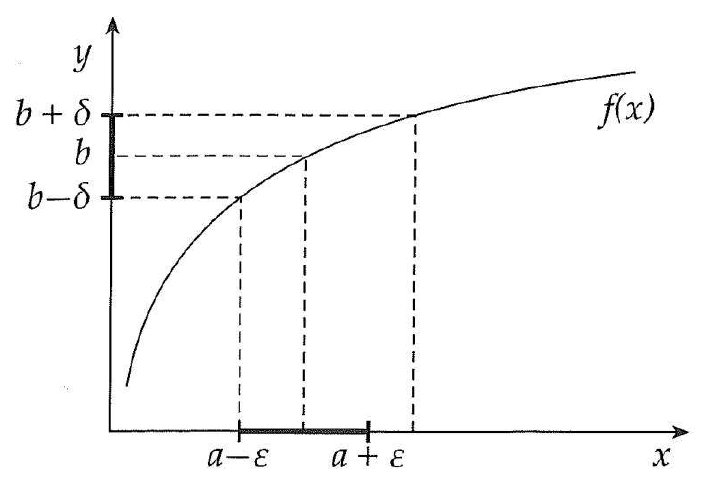
\includegraphics[scale=0.3]{images/figure_01_12.png} \end{figure}

As in the case of successions, where the value of $N$ depends on the value of $\delta$, the value of $\varepsilon$ also depends on the value of $\delta$. Usually, the closer we want to be to $\textbf{b}$ (the smaller the $\delta$) the closer will $\textbf{x}$ need to be to $\textbf{a}$ (the smaller will $\varepsilon$ have to be), to guarantee that $\textbf{f(x)}$ is in the neighborhood of $\textbf{b}$.


\noindent\rule{\textwidth}{1pt}

$\textbf{Definition 1.1}$ Let $\textbf{a} \in D$ be an accumulation point of the domain of function $\textbf{f}: D \subseteq \mathbb{R}^n \to \mathbb{R}^m$. It is said that $\textbf{b} \in \mathbb{R}^m$ is the limit of $\textbf{f}$ in point $\textbf{a}$ (or the limit of $\textbf{f}$ when $\textbf{x}$ tends to $\textbf{a}$) and is written as $\lim_{\textbf{x}\to \textbf{a}}=\textbf{b}$, if, for any $\delta >0$, exists a $\varepsilon >0$, such that $\norm{\textbf{f}(\textbf{x})-\textbf{b}}<\delta$ for all points, such that $0<\norm{\textbf{x}-\textbf{a}}<\varepsilon, \textbf{x}\in D$. Written in another way: 
$$ \lim_{\textbf{x}\to \textbf{a}} \textbf{f}(\textbf{x}) =\textbf{b} \equiv \forall \delta>0, \exists\varepsilon>0:\textbf{x}\in(B_\varepsilon(\textbf{a})\setminus\{\textbf{a}\})\cap D \Rightarrow \textbf{f}(\textbf{x}) \in B_\delta(\textbf{b}) $$
$\noindent\rule{\textwidth}{1pt}$

$\textbf{Theorem 1.1}$ The limit of $\textbf{f}$ in point $\textbf{a}$, when it exists, is unique.

$\textbf{Proof}$ As usual in results of singleness, this theorem can be proven by reduction to absurdity. Let us suppose that exist two different limits $\textbf{b}_1$ and $\textbf{b}_2$. If this were the case, we could always choose the neighborhoods $\delta_1$ and $\delta_2$ of these points, such that $V_{\delta_1}(\textbf{b}_1)\cap V_{\delta_2}(\textbf{b}_2) = \emptyset$ (we could choose $\delta_1 = \delta_2 < \norm{(\textbf{b}_2-\textbf{b}_1)/2}$). By the definition of limit at $\textbf{a}$, if $\textbf{b}_1$ was to be the limit of the function in that point, then $\exists\varepsilon_1>0:\textbf{x}\in(B_{\varepsilon_1}(\textbf{a})\setminus\{\textbf{a}\})\cap D \Rightarrow \textbf{f}(\textbf{x}) \in B_{\delta_1}(\textbf{b}_1)$. The same way, if $\textbf{b}_2$ was to be the limit of the function in that point, then $\exists\varepsilon_2>0:\textbf{x}\in(B_{\varepsilon_2}(\textbf{a})\setminus\{\textbf{a}\})\cap D \Rightarrow \textbf{f}(\textbf{x}) \in B_{\delta_2}(\textbf{b}_2)$. By choosing the smallest between $\varepsilon_1$ and $\varepsilon_2$ results that if $\textbf{x} \in V_{\text{min}\{\varepsilon_1,\varepsilon_2\}}(\textbf{a})\setminus\{\textbf{a}\}$, then $\textbf{f}(\textbf{x}) \in V_{\delta_1}(\textbf{b}_1)\cap V_{\delta_2}(\textbf{b}_2)$. This result is absurd because $V_{\delta_1}(\textbf{b}_1)\cap V_{\delta_2}(\textbf{b}_2)=\emptyset$.

\noindent\rule{\textwidth}{1pt}

$\textbf{Theorem 1.2}$ $\lim_{\textbf{x}\to\textbf{a}} \textbf{f}(\textbf{x})=\textbf{b}$, if and only if, for each succession of ($\textbf{x}_n$) of limit $\textbf{a}$, and made up of elements of the domain of the function distinct of $\textbf{a}$, the corresponding succession $\textbf{f}(\textbf{x})$ tends to $\textbf{b}$.

$\textbf{Proof}$ As we are dealing with an equivalence, the demonstration can be made by showing that when the first proposition is true, so is the second, and when it is false, the second is also false.

Let us see the first part. As the limit of the function at $\textbf{a}$ is $\textbf{b}$, we know that, whatever the value for $\delta$, there exists a $\varepsilon$ such that $0<\norm{\textbf{x}_n-\textbf{a}}<\varepsilon \Rightarrow \norm{\textbf{f}(\textbf{x}_n)-\textbf{b}}<\delta$. Consider a succession ($\textbf{x}_n$) that converges to $\textbf{a}$ (and that $\textbf{x}_n\neq\textbf{a}$). By the definition of the limit of a succession, we know that, whichever $\varepsilon>0$, there exists an order from which on all the terms of the succession are in the neighborhood $\varepsilon$ of $\textbf{a}$. Or formally, $\forall\varepsilon, \exists N:n\geq N \Rightarrow 0< \norm{\textbf{x}_n-\textbf{a}}<\varepsilon$. In this case, we verify that if $n\geq N$ then $0< \norm{\textbf{x}_n-\textbf{a}}<\varepsilon$ and $0< \norm{\textbf{x}_n-\textbf{a}}<\varepsilon \Rightarrow \norm{\textbf{f}(\textbf{x}_n)-\textbf{b}}<\delta$. By transitivity, $n\geq N \Rightarrow \norm{\textbf{f}(\textbf{x}_n)-\textbf{b}}<\delta$, which confirms that $\textbf{f}(\textbf{x}_n)$ converges to $\textbf{b}$.

With regards to the second part, we want to show that it is possible to find a succession ($\textbf{x}_n$) that tends to $\textbf{a}$ (and with $\textbf{x}_n \neq \textbf{a}$) without the succession of $\textbf{f}(\textbf{a})$ converging to $\textbf{b}$. Saying $\lnot (\lim_{\textbf{x}\to \textbf{a}} \textbf{f}(\textbf{x})=\textbf{b})$ is equivalent to affirming that exists a $\delta$, such that, whichever $\varepsilon>0$, we have $0<\norm{\textbf{x}_n-\textbf{a}}<\varepsilon$ and, simultaneously, $\norm{\textbf{f}(\textbf{x}_n)-\textbf{b}}\geq \delta$. But, in this case, we can choose for any natural number $n$ a point $\textbf{x}_n\in D\setminus\{\textbf{a}\}$, such that $0<\norm{\textbf{x}_n-\textbf{a}}<1/n$ and $\norm{\textbf{f}(\textbf{x}_n)-\textbf{b}}\geq \delta$. This means that the succession ($\textbf{x}_n$) converges to $\textbf{a}$ but the corresponding succession of $\textbf{f}(\textbf{x}_n)$ does not converge to $\textbf{b}$.

\noindent\rule{\textwidth}{1pt}

$\textbf{Theorem 1.3}$ Considering $\textbf{f}$ and $\textbf{g}$ functions that take values in $\mathbb{R}^m$, and $h$ a function that takes values in $\mathbb{R}$ (real function), all of them with domain $D \subseteq \mathbb{R}^n$. If these functions have limit at $\textbf{a}$, then:
\begin{enumerate}
	\item $\lim_{\textbf{x}\to\textbf{a}} [\textbf{f}(\textbf{x})+\textbf{g}(\textbf{x})] = \lim_{\textbf{x}\to\textbf{a}} \textbf{f}(\textbf{x}) + \lim_{\textbf{x}\to\textbf{a}} \textbf{g}(\textbf{x})$;
	\item $\lim_{\textbf{x}\to\textbf{a}} [h(\textbf{x})\textbf{f}(\textbf{x})] = \lim_{\textbf{x}\to\textbf{a}} h(\textbf{x}) \lim_{\textbf{x}\to\textbf{a}} \textbf{f}(\textbf{x})$;
	\item $\lim_{\textbf{x}\to\textbf{a}} \norm{\textbf{f}(\textbf{x})} = \norm{\lim_{\textbf{x}\to\textbf{a}} \textbf{f}(\textbf{x})}$;
	\item $\lim_{\textbf{x}\to\textbf{a}}[\textbf{f}(\textbf{x})\cdot\textbf{g}(\textbf{x})]=[\lim_{\textbf{x}\to\textbf{a}} \textbf{f}(\textbf{x})]\cdot [\lim_{\textbf{x}\to\textbf{a}} \textbf{g}(\textbf{x})]$.
\end{enumerate}	

\noindent\rule{\textwidth}{1pt}

$\textbf{Theorem 1.4}$ Considering $\textbf{g}$ a function of domain $A \subseteq \mathbb{R}^n$ and codomain  $\textbf{g)(A)}$, with $\textbf{g)(A)} \subseteq B \subseteq \mathbb{R}^m$ and $\textbf{f}$ a function of domain $B$ and taking values in $\mathbb{R}^p$. Let us designate $\textbf{u}=\textbf{f} \circ \textbf{g} $ as a composite function of $\textbf{g}$ and $\textbf{f}$ ($\textbf{u}$ has domain $A$ and takes values in $\mathbb{R}^p$). If $\lim_{\textbf{x}\to\textbf{a}} \textbf{g}(\textbf{x})=\textbf{b}$ and $\lim_{\textbf{y}\to\textbf{b}} \textbf{f}(\textbf{y})=\textbf{c}$ then we have $\lim_{\textbf{x}\to\textbf{a}} \textbf{u}(\textbf{x})=\lim_{\textbf{x}\to\textbf{a}} \textbf{f}(\textbf{g}(\textbf{x}))=\textbf{c}$.

$\textbf{Proof}$ To show this result we use the equivalence between the existence of limit of a function in a point and the convergence of a succession of images, always considering a succession of points of the domain towards $\textbf{a}$. We know then that $\lim_{\textbf{x}\to\textbf{a}} \textbf{g}(\textbf{x})=\textbf{b}$, that is, $\forall(\textbf{x}_n)\neq\textbf{a}$ such that $\lim_{n\to\infty} \textbf{x}_n=\textbf{a}$, then $\lim_{n\to
\infty}\textbf{g}(\textbf{x}_n)=\textbf{b}$. Identically, $\lim_{\textbf{g}(\textbf{x})\to\textbf{b}}\textbf{f}(\textbf{g}(\textbf{x}))=\textbf{c}$, that is, $\forall(\textbf{g}(\textbf{x}))\neq\textbf{b}$ such that $\lim_{n\to\infty}\textbf{g}(\textbf{x}_n)=\textbf{b}$, then $\lim_{n\to\infty}\textbf{f}(\textbf{g}(\textbf{x}_n))=\textbf{c}$. Meaning that $\lim_{n\to\infty}\textbf{x}_n=\textbf{a}\Rightarrow\lim_{n\to\infty}\textbf{f}(\textbf{g}(\textbf{x}_n))=\textbf{c}$, which in turn is equivalent to saying that the limit of the composite function when $\textbf{x}$ tends to $\textbf{a}$ is equal to $\textbf{c}$.



\addcontentsline{toc}{subsection}{1.5 Continuity}
\subsection*{1.5 Continuity}



$\textbf{Definition 1.2}$ Consider $\textbf{a}$ a point of the domain of the function $\textbf{f}: D\subseteq \mathbb{R}^n\to\mathbb{R}^m$. The function is continuous at point $\textbf{a}$ if, for all $\delta>0$, exists an $\varepsilon>0$, such that $\norm{\textbf{f}(\textbf{x})-\textbf{f}(\textbf{a})}<\delta$, whenever $\norm{\textbf{x}-\textbf{a}}<\varepsilon$, $\textbf{x}\in D$.

\noindent\rule{\textwidth}{1pt}

One should note that in this definition we do not impose that $\textbf{x}$ be different than $\textbf{a}$, as it happens in the definition of a limit. Moreover, the $\textbf{a}$ may or not be an accumulation point. Lastly, in this case there is the requisite that $\textbf{f}(\textbf{x})$ be in the neighborhood of $\textbf{f}(\textbf{a})$ instead of $\textbf{b}$.

\noindent\rule{\textwidth}{1pt}

$\textbf{Definition 1.3}$ Consider $\textbf{a}\in D$ an accumulation point of the domain $D$ of the function $\textbf{f}:D\subseteq \mathbb{R}^n \to \mathbb{R}^m$. A function is said to be continuous at $\textbf{a}$ if $\lim_{\textbf{x}\to \textbf{a}} \textbf{f}(\textbf{x})  = \textbf{f}(\textbf{a})$. By other words, the limit of the function at a certain point is equal to the value of the function in that point. 

\noindent\rule{\textwidth}{1pt}

When do we say that a function is continuous? When it is continuous in all the points of its domain.

\noindent\rule{\textwidth}{1pt}

$\textbf{Theorem 1.5}$ Consider the functions $\textbf{f}$ and $\textbf{g}$ with values in $\mathbb{R}^m$, and $h$ a function with values in $\mathbb{R}$, all with domain $D\subseteqq\mathbb{R}^n$. Then, if $\textbf{f}$, $\textbf{g}$, and $h$ are continuous in $\textbf{a}\in D$, the same happens with
$$\textbf{f}+\textbf{g},\ \textbf{g}\cdot\textbf{f},\ \norm{\textbf{f}},\ h\textbf{f},\ \text{and }\frac{1}{h}\textbf{f}\text{ as long as }h(\textbf{a})\neq0$$

\noindent\rule{\textwidth}{1pt}

$\textbf{Theorem 1.6}$ A vector function $\textbf{f}:D\subseteq\mathbb{R}^n\to\mathbb{R}^m$ (with $m>1$) is continuous at $\textbf{a}$ if and only if $f_1:D\subseteq\mathbb{R}^n\to\mathbb{R}, f_2:D\subseteq\mathbb{R}^n\to\mathbb{R}, \dots, f_m:D\subseteq\mathbb{R}^n\to\mathbb{R}$ are continuous at $\textbf{a}$.

$\textbf{Proof}$ As the result presents us with an equivalence, we have to demonstrate the implication in both directions. First, if the vector function is continuous then each of its coordinates also is continuous. Consider $\textbf{e}_k$ the k-nth vector of the canonical base of $\mathbb{R}^m$. As $f_k(\textbf{x})=\textbf{f}(\textbf{x})\cdot \textbf{e}_k$, we have that $\lim_{\textbf{x}\to\textbf{a}}f_k(\textbf{x})=\lim_{\textbf{x}\to\textbf{a}}\textbf{f}(\textbf{x})\cdot\lim_{\textbf{x}\to\textbf{a}}\textbf{e}_k$, by the theorem of the limit of the product of two functions. This in turn implies that $\lim_{\textbf{x}\to\textbf{a}}f_k(\textbf{x})=\textbf{f}(\textbf{a})\cdot\textbf{e}_k=f_k(\textbf{a})$. As this is true for all $k$, it is then demonstrated that the continuity of the function implies the continuity of each component. On the other hand, given that $\textbf{f}(\textbf{x})=\sum_{k=1}^{m}f_k(\textbf{x})\cdot\textbf{e}_k$ and using the theorem of the sum and the product, we can conclude that if all components $f_k$ are continuous then the function also is continuous.

\noindent\rule{\textwidth}{1pt}

$\textbf{Theorem 1.7}$ A function is continuous at $\textbf{a}$ if and only if for each succession $(\textbf{x}_n)$ formed by elements of the domain of the converging function to $\textbf{a}$, the corresponding converging function $\textbf{f}(\textbf{x}_n)$ converges to $\textbf{f}(\textbf{a})$.


\noindent\rule{\textwidth}{1pt}

$\textbf{Theorem 1.8}$ If $\textbf{g}:A\subseteq\mathbb{R}^n\to\mathbb{R}^m$ is continuous at $\textbf{a}\in A$ and $\textbf{f}:B\subseteq\mathbb{R}^m\to\mathbb{R}^p$ is continuous at $\textbf{b}=\textbf{g}(\textbf{a})$, then the composite function $\textbf{u}=\textbf{f}\circ\textbf{g}$ is continuous at $\textbf{a}$.

\noindent\rule{\textwidth}{1pt}

$\textbf{Theorem 1.9}$ If $\textbf{f}:D\subseteq\mathbb{R}^n\to\mathbb{R}^m$ is continuous in a compact set $X\subseteq D$, then $\textbf{f}(X)$ is compact in $\mathbb{R}^m$.

$\textbf{Proof}$ A set is compact if any succession of elements of the set has a sub-succession that converges to an element of the set. In this scenario, we have to prove that any succession of elements of $\textbf{f}(X)$ (the image of the set $X$) has a sub-succession that converges to an element of $\textbf{f}(X)$. Consider any succession of points ($\textbf{y}_n$) in $\textbf{f}(X)$. Then, there exists ($\textbf{x}_n$) such that $\textbf{y}_n=\textbf{f}(\textbf{x}_n)$, with $\textbf{x}_n \in X$. We know that there is a sub-succession ($\textbf{x}_{n_k}$) convergent to a point $\textbf{a}$ of $X$ (as the set is compact). This implies that $\textbf{y}_{n_k}=\textbf{f}(\textbf{x}_{n_k})\to\textbf{f}(\textbf{a})$ (as the function is continuous and there is equivalence between and convergence of the succession of corresponding images). That is, we can conclude that $\textbf{y}_{n_k}$ is a sub-succession that converges to $\textbf{f}(\textbf{a})$. So, $\textbf{f}(X)$ is a compact set.

\noindent\rule{\textwidth}{1pt}

$\textbf{Theorem 1.10}$ If $\textbf{f}:D\subseteq\mathbb{R}^n\to\mathbb{R}^m$ is continuous in a connected set $X\subseteq D$, then $\textbf{f}(X)$ is a connected set

\noindent\rule{\textwidth}{1pt}

$\textbf{Theorem 1.11}$ Consider $f:D\subseteq\mathbb{R}^n\to\mathbb{R}$ a continuous function at point $\textbf{a}$, an interior point of the domain of te function. If $f(\textbf{a})\neq0$, then there is a ball of center $\textbf{a}$ in which the function has the same sign as in $f(\textbf{a})$.

$\textbf{Proof}$ Admit that $f(\textbf{a})>0$ (the proof for the contrary is similar). We know that the function is continuous and we want to prove that there is a neighborhood of $\textbf{a}$ for which the function takes positive values. Let us choose a neighborhood $\delta$ of $f(\textbf{a})$ such that all points in its neighborhood are positive. For example, if $\delta=f(\textbf{a})/2$, the neighborhood is given by $]f(\textbf{a})-f(\textbf{a})/2,f(\textbf{a})+f(\textbf{a})/2[$. But, if the function is continuous then there must exist, for this $\delta$, a neighborhood $\varepsilon$ of point $\textbf{a}$, such that $\norm{\textbf{x}-\textbf{a}}<\varepsilon\Rightarrow\abs{f(\textbf{x})-(\textbf{a})}<f(\textbf{a})/2]$. That is, $f(\textbf{a})/2<f(\textbf{x})<3f(\textbf{a})/2$, in which $f(\textbf{x})>0$ as we assumed that $f(\textbf{a})>0$.

\clearpage

\addcontentsline{toc}{section}{2 Differentiability}
\section*{2 Differentiability}
\addcontentsline{toc}{subsection}{2.1 Differentiability of a real function of a real variable}
\subsection*{2.1 Differentiability of a real function of a real variable}

$\textbf{Definition 2.1}$ Consider $f$ a real function of real variable, and $\textbf{a}$ an interior point of the domain. The derivative of function $f$ at point $\textbf{a}$ is the following limit (when it exists):
$$\lim_{h\to0}\frac{f(a+h)-f(a)}{h},$$
and is designated as $f'(a),\ df/dx(a),\ \left( df/dx \right)_{x=a},\ \text{or }(Df)(a)$. To the lateral limits:
$$\lim_{h\to0^+}\frac{f(a+h)-f(a)}{h}\quad\text{and}\quad\lim_{h\to0^-}\frac{f(a+h)-f(a)}{h},$$
we call lateral partial derivatives (when $h\to0^+$, we have the right partial derivative, and when $h\to0^-$, we have the left partial derivative).

\noindent\rule{\textwidth}{1pt}

$\textbf{Definition 2.2}$ Consider $f$ a real function of real variable, and $a$ an interior point of the domain. The function $f$ is differentiable at $a$ if there is a line that passes through the point $(a,f(a))$, with equation $y=f(a)+\alpha(x-a)$ such that the difference $f(x)-y$ is an infinitesimal of order superior to $(x-a)$. That is, 
$$\lim_{x\to a} \frac{f(x)-y}{x-a}=0.$$ 

\noindent\rule{\textwidth}{1pt}

If the function is differentiable at $a$, in a neighborhood of that point, it can be represented as:
$$f(x)=f(a)+f'(a)(x-a)+o(\abs{x-a})\quad\text{or}\quad f(x)-f(a)=f'(a)(x-a)+o(\abs{x-a}),$$
where the notation $o(g)$ means an infinitesimal of order superior to $g$.

\addcontentsline{toc}{subsection}{2.2 Partial Derivatives}
\subsection*{2.2 Partial Derivatives}

$\textbf{Definition 2.3}$ Consider $\textbf{a}=(a_1,a_2, \dots, a_n)$ an interior point of the domain of a function $f:D\subseteq\mathbb{R}^n\to\mathbb{R}$. The partial derivative at $\textbf{a}$ with regards to $x_i$ is given by the limit (when it exists):
$$\lim_{h\to0}\frac{f(a_1,\dots,a_{i-1},a_i+h,a_{i+1},\dots,a_n)-f(a_1,\dots,a_{i-1},a_i,a_{i+1},\dots,a_n)}{h},$$ 
and is usually called $\partial f/\partial x_i(\textbf{a}),\  f_{x_i}(\textbf{a}),\ (D_i f)(\textbf{a}),\ \text{or }f'_{x_i}$.

\noindent\rule{\textwidth}{1pt}

Consider $f$ a real function of real variables. To the vector of all partial derivatives of $f$ we call the gradient of the function. On the other hand, consider $\textbf{f}:\mathbb{R}^n\to\mathbb{R}^m$. We call Jacobian matrix of function $\textbf{f}$ at $\textbf{a}$ to the matrix $m\times n$ of partial derivatives evaluated at $\textbf{a}$.

\addcontentsline{toc}{subsection}{2.3 Derivatives of higher order and the hessian matrix}
\subsection*{2.3 Derivatives of higher order and the hessian matrix}

We call the derivative of $f'_x$ the derivative of second order of function $f$, and represent it as $f''_x, \partial^2f/\partial x^2,\text{ or }D^2f$. The second order derivative indicates the curvature of the function.

Consider $f:\mathbb{R}^n\to\mathbb{R}$ a real function of real variables. The matrix of partial derivatives of second order  of a real function of real variables is called hessian matrix, and it is always $n\times n$.


\addcontentsline{toc}{subsection}{2.4 Derivative of a function at a point along a vector}
\subsection*{2.4 Derivative of a function at a point along a vector}

$\textbf{Definition 2.4}$ Consider $f:D\subseteq\mathbb{R}^n\to\mathbb{R}$, $\textbf{a}$ an interior point of the domain, and $\textbf{u}$ a vector in $\mathbb{R}^n$. We call the derivative of $f$ at $\textbf{a}$ along vector $\textbf{u}$ to the limit (when it exists):
$$\lim_{t\to0}\frac{f(\textbf{a}+t\textbf{u})-f(\textbf{a})}{t},$$
which is commonly represented as $f'_\textbf{u}(\textbf{a})$ or $D_\textbf{u}f(\textbf{a})$. The derivative along a vector is also called directional derivative. If the norm of the vector $\textbf{u}$ is $1$, then the derivative along a vector is called $\textit{derivada dirigida}$.

\addcontentsline{toc}{subsection}{2.5 Differentiability}
\subsection*{2.5 Differentiability}

For real functions of real variable, if a function has partial derivative in a point, then it is continuous. In $\mathbb{R}^n$, all directional derivative might exist at a point and yet the function might not be continuous. The reason is that the existence of all directional derivatives does not imply continuity at that point: $\exists \lim_{\textbf{x}\to\textbf{a}}f(\textbf{x})\not\Rightarrow\lim_{\textbf{x}\to\textbf{a}}f(\textbf{x})=f(\textbf{a})$.

The function $f:\mathbb{R}\to\mathbb{R}$ is differentiable if it can be locally approximated with a tangent line to the curve at a point (with an approximation error an infinitesimal of superior order to $\abs{x-a}$, the deviation to the point). In $\mathbb{R}^n$, we have an hyperplane instead of a straight line. The function $f:\mathbb{R}^n\to\mathbb{R}$ is differentiable if it can be locally approximated by an hyperplane that is tangent to the function at a point (where, once again, the error ought to be way smaller when compared to the deviation to the point).

\noindent\rule{\textwidth}{1pt}

$\textbf{Definition 2.5}$ Consider $\textbf{a}=(a_1, a_2)$ an interior point of the domain of $f:D\subseteq\mathbb{R}^2\to\mathbb{R}$. The function $f$ is differentiable at $\textbf{a}$ when, in some neighborhood of the point, the function can be represented as:
$$f(a_1+u_1, a_2+u_2)=\alpha_1x_1+\alpha_2x_2 +\gamma+\varepsilon\rho,$$
where $\alpha_1,\ \alpha_2,\ \gamma$ are real constants, $\rho=\norm{\textbf{u}}=\sqrt{u_1^2+u_2^2}$, and $\lim_{\rho\to0}\varepsilon=0$.

\noindent\rule{\textwidth}{1pt}

From this definition we can conclude that:
\begin{enumerate}
	\item If the function is differentiable at $\textbf{a}$, then $\gamma=f(\textbf{a})$.
	\item If the function is differentiable at $\textbf{a}$, then it is continuous at that point.
	\item If the function is differentiable at $\textbf{a}$, then it has partial partial derivatives at that point.
\end{enumerate}

In turn, we can rewrite the expression as:
$$f(a_1+u_1, a_2+u_2)=f(a_1,a_2)+f'_{x_1}(a_1,a_2)u_1 + f'_{x_2}(a_1,a_2)u_2+o(\rho).$$ 
We can replace $\varepsilon\rho$ by $o(\rho)$. But why? If we calculate $\lim_{\rho\to0}\varepsilon\rho\rho$, we obtain $\lim_{\rho\to0}\varepsilon$, but $\lim_{\rho\to0}\varepsilon=0$ by the definition of differentiable function. This, in fact, implies that $\varepsilon$ is an infinitesimal order superior to $\rho$.

Also, instead of using the deviations vector $\textbf{u}=(u_1,u_2)$, we can define $\textbf{x}=(x_1,x_2)=(a_1,a_2)+(u_1,u_2)$ and rewrite the expression as:
$$f(x_1,x_2)=f(a_1,a_2)+f'{x_1}(a_1,a_2)(x_1-a_1)+f'{x_2}(a_1,a_2)(x_2-a_2)+o(\rho)$$
where $\rho=\sqrt{(x_1-a_1)^2+(x_2-a_2)^2}$.

Considering a plane in $\mathbb{R}^3$ that passes through $\textbf{a}=(a_1,a_2,a_3)$ and whose normal vector is $\textbf{u}=(u_1,u_2,u_3)$. We can use the fact that $\textbf{u}$ has to be orthogonal to any vector in the plane to determine the equation of said plane: $ \textbf{x}\cdot(\textbf{x}-\textbf{a}) =0$. 

If $u_3$, we can define $\alpha_1=-u_1/u_3$ and $\alpha_2=-u_2/u_3$ so that: $x_3=a_3+\alpha_1(x_1-a_1)+\alpha_2(x_2-a_2)$. We can determine the equation of the plane tangent to the function at $(a_1,a_2;f(a_1,a_2))$ by using the fact that the tangent lines to the plane belong to the tangent plane when $x_1=a_1$ and $x_2=a_2$. Therefor, we have: $y=f(a_1,a_2)+\alpha_1(x_1-a_1)+\alpha_2(x_2-a_2)$. By knowing that tangent line to the function when $x_2=a_2$ is given by $y=f(a_1,a_2)+f'{x_1}(a_1,a_2)(x_1-a_1)$, for this straight line to belong to the plane, then $\alpha_1$ has to be equal to $f'{x_1}(a_1,a_2)$. The same logic applies to $\alpha_2$. We then get to the equation of the plane tangent to the function $f(x_1, x_2)$ at $(\textbf{a}, f(\textbf{a}))$:
$$y=f(a_1,a_2)+f'{x_1}(a_1,a_2)(x_1-a_1)+f'{x_2}(a_1,a_2)(x_2-a_2).$$
It can also be represented in the following matrix notation:
$$ y = f(\textbf{a})+\nabla f(\textbf{a})\cdot(\textbf{x}-\textbf{a})$$.
Note the resemblance to the equation of the tangent line of a real function of real variable: $y=f(a)+f'(a)(x-a)$.

The matrix representation of the neighborhood of a function is that is differentiable in a point is:
$$f(\textbf{a}+\textbf{u})-f(\textbf{a})=\nabla f(\textbf{a})\cdot\textbf{u}+o(\rho).$$
The left side of this equation, $f(\textbf{a}+\textbf{u})-f(\textbf{a})$, is the increase of the function between $\textbf{a}$ and $\textbf{a}+\textbf{u}$. The expression $\nabla f(\textbf{a})\cdot\textbf{u}$ is the differential of function $f$ at $\textbf{a}$ along $\textbf{u}$, or $d_uf(\textbf{a})$. If the function is differentiable, then the difference between the increase and the differential will be an infinitesimal of order superior to $\rho$.

The interpretation tells us that: if we move a small distance away from $\textbf{a}$, the value of the value of the differential is a good approximation of the increase of the function. That is, the differential is an approximated value of the increase of the function. If instead of thinking about a specific point and direction we think in generic terms, the differential is given by $df=f'_{x_1}u_1+f'_{x_2}u_2$.

\noindent\rule{\textwidth}{1pt}

$\textbf{Definition 2.6}$ Consider $\textbf{a}$ an interior point of the domain of $f:D\subseteq\mathbb{R}^n\to\mathbb{R}$. The function $f$ is said to be differentiable at $\textbf{a}$ when, in a neighborhood of this point, the function can be written as:
$$f(\textbf{a}+\textbf{u})=\alpha_1u_1+\alpha_2u_2+\dots+\alpha_nu_n+\gamma+\varepsilon\rho,$$
where $\alpha_1,\ \alpha_2,\dots,\ \alpha_n,\ \text{and }\gamma$ are real constants, $\rho=\norm{\textbf{u}}=\sqrt{u_1^2+\dots+u_n^2}$, and $lim_{\rho\to0}\varepsilon=0$.

\noindent\rule{\textwidth}{1pt}

Once again, given previous observations, the matrix representation is given by:
$$f(\textbf{a}+\textbf{u})=f(\textbf{a})+\nabla f(\textbf{a})\cdot\textbf{u}+o(\rho).$$
The geometric interpretation is that the function is differentiable at $\textbf{a}$ if there is an hyperplane that is tangent to the function at $\textbf{a}$ and whose local approximation is good. The equation of the plane is $y=f(\textbf{a})+\nabla f(\textbf{a})$ and $o(\rho)$ is the error of the approximation.

The expression $\nabla f(\textbf{a})\cdot\textbf{u}$ is the differential of the function at $\textbf{a}$ along $\textbf{u}$. When $\norm{\textbf{u}}$ tends to $0$ (when we get very little away from $\textbf{a}$), the value of the differential tends to the value of the increase at a superior rate than $\norm{\textbf{u}}$ is converging to $0$. In this scenario (in which we get ever so little away from $\textbf{a}$), we can evaluate the function by using the fact that $\textbf{x}=\textbf{a}+\textbf{u}$:
$$f(\textbf{x})=f(\textbf{a})+\nabla f(\textbf{a})(\textbf{x}-\textbf{a})+o(\rho).$$

\noindent\rule{\textwidth}{1pt}

$\textbf{Definition 2.7}$ Consider $\textbf{a}$ an interior point of the domain of $\textbf{f}:D\subseteq\mathbb{R}^n\to\mathbb{R}^m$. The function $f$ is differentiable at $\textbf{a}$ when, in some neighborhood of this point, the function can be represented as:
$$\textbf{f}(\textbf{a}+\textbf{u})=L_\textbf{a}\textbf{u}+\gamma+\epsilon,$$
where $L_\textbf{a}$ is a linear operator of $\mathbb{R}^n\to\mathbb{R}^m$ (it transforms vector of $\mathbb{R}^n$ to $\mathbb{R}^m$, as it is a $m\times n$ matrix) that is independent of $\textbf{u}$, $\gamma$ is a $m\times1$ vector of real constants, and $\varepsilon$ is a vector of infinitesimals of order superior to $\rho=\norm{u}$.

\noindent\rule{\textwidth}{1pt}

With vector functions, $L_\textbf{a}$ is the jacobian matrix evaluated at $\textbf{a}$, and $\gamma$ is the vector of images of $\textbf{f}$ at $\textbf{a}$.

\noindent\rule{\textwidth}{1pt}

$\textbf{Theorem 2.1}$ A vector function, $\textbf{f}$, is differentiable at $\textbf{a}$, if and only if each component $f_i$ is differentiable at $\textbf{a}$.

$\textbf{Proof}$ The above representation is equivalent to:
$$
\begin{bmatrix}
f_1(\textbf{a}+\textbf{u})\\ 
f_2(\textbf{a}+\textbf{u})\\
\vdots \\
f_n(\textbf{a}+\textbf{u})\\
\end{bmatrix}
=
\begin{bmatrix}
f_1(\textbf{a})\\ 
f_2(\textbf{a})\\
\vdots \\
f_n(\textbf{a})\\
\end{bmatrix}
+
\begin{bmatrix}
\frac{\partial f_1}{\partial x_1}(\textbf{a}) & \frac{\partial f_1}{\partial x_2}(\textbf{a}) & \dots & \frac{\partial f_1}{\partial x_n}(\textbf{a})\\ 
\frac{\partial f_2}{\partial x_1}(\textbf{a}) & \frac{\partial f_2}{\partial x_2}(\textbf{a}) & \dots & \frac{\partial f_2}{\partial x_n}(\textbf{a}) \\ 
\vdots & \vdots & \ddots & \vdots \\ 
\frac{\partial f_m}{\partial x_1}(\textbf{a}) & \frac{\partial f_m}{\partial x_2}(\textbf{a}) & \dots & \frac{\partial f_m}{\partial x_n}(\textbf{a})
\end{bmatrix}
\begin{bmatrix}
u_1\\ 
u_2\\
\vdots \\
u_n\\
\end{bmatrix}
+
\begin{bmatrix}
o_1(\rho)\\ 
o_2(\rho)\\
\vdots \\
o_n(\rho)\\
\end{bmatrix}.
$$
By doing the algebra, we verify the equality of two vectors, if and only if all coordinates are equal. As the equality of the i-nth coordinates of the two vectors corresponds to saying that the function $ f_i $ is differentiable, the equivalence is then proved.

\noindent\rule{\textwidth}{1pt}

$\textbf{Theorem 2.2}$ A real function of $n$ variables that has partial derivatives of first order is differentiable in all points where $n-1$ of the partial derivatives are continuous.

$\textbf{Proof}$ We start by rewriting $f(a+h,b+k)-f(a,b)$ as $\left[ f(a+h,b)-f(a,b) \right]+\left[ f(a+h,b+k)-f(a+h,b) \right]$. By using the definition of partial derivative we get: $(a+h,b+k)-f(a,b) = h\left[f'_x(a,b)+\varepsilon_1 \right] + k\left[f'_y(a+h,b)+\varepsilon_2\right]$, where $\lim_{h\to0}\varepsilon_1=0$ and $\lim_{h\to0}\varepsilon_2=0$. Notice that $f'_y$ is evaluated at $(a+h,b)$. Let us admit that the partial derivative in order to $y$ is continuous at $(a,b)$. If this were to happen, we would verify that $f'_y(a+h,b)=f'_y(a,b)+\varepsilon_3$, with $\lim_{h\to0}\varepsilon_3=0$. If we substitute in the last expression we get: $f(a+h,b+k)-f(a,b)=hf'_x(a,b)+kf'_y(a,b)+h\varepsilon_1+k(\varepsilon_2+\varepsilon_3)$. To know if this function is differentiable, we must verify if $h\varepsilon_1+k(\varepsilon_2+\varepsilon_3)$ is an infinitesimal of order superior to $p=\sqrt{h^2+k^2}$. We have to verify if $\lim_{\rho\to0}\abs{h\varepsilon_1+k(\varepsilon_2+\varepsilon_3)}/\rho=0$. We know that:
$$\abs{h\varepsilon_1+k(\varepsilon_2+\varepsilon_3)}/\rho\leq\abs{\varepsilon_1}\cdot\abs{\frac{h}{\rho}}+\abs{\varepsilon_2+\varepsilon_3}\cdot\frac{k}{\rho}\leq\abs{\varepsilon_1}+\abs{\varepsilon_2}+\abs{\varepsilon_3}.$$
As $\abs{\varepsilon_1},\ \abs{\varepsilon_2},\ \text{and }\abs{\varepsilon_3}$ all converge to zero when $\rho$ tends to zero, it is proved that that $h\varepsilon_1+k(\varepsilon_2+\varepsilon_3)$ is an infinitesimal of order superior to $\rho$. Thus, this function is differentiable.

\noindent\rule{\textwidth}{1pt}

$\textbf{Definition 2.8}$ A function $f$ is of class $C^r$ at $S$ when it admits continuous partial derivatives until order $r$, in all points of the set $S$.

\noindent\rule{\textwidth}{1pt}

$\textbf{Theorem 2.3}$ All functions of class $C^1$ are differentiable.

\noindent\rule{\textwidth}{1pt}

If a function is of class $C^1$, then all its partial derivatives are continuous. Given that we only need $n-1$ partial derivatives for a function to be differentiable, this function is therefor differentiable.

When we talk about the directional derivative, we say that it is equal to the slope of a tangent line to the function at that point, in turn a straight line in the perpendicular direction. On the other hand, if the function is differentiable, it can be approximated by a hyperplane tangent to the function at the point. The existence of this plane implies that all tangent lines to the function must lie on top of it. Or, in other words, if the function is differentiable at a point, whatever directional partial derivative at that point may be written as a combination of partial derivatives.

\noindent\rule{\textwidth}{1pt}

$\textbf{Theorem 2.4}$ If a function $f:D\subseteq\mathbb{R}^n\to\mathbb{R}$ is differentiable at $\textbf{a}$, then the partial derivative along the vector $\textbf{u}$ can be written as a combination of the partial derivatives. That is:
$$f'_\textbf{u}(\textbf{a})=f'_{x_1}(\textbf{a})u_1+f'_{x_2}(\textbf{a})u_2+\dots+f'_{x_n}(\textbf{a})u_n=\nabla f(\textbf{a})\cdot\textbf{u}$$

$\textbf{Proof}$ By definition, the partial derivative along $\textbf{u}$ at $\textbf{a}$ is given by: $f'_\textbf{u}(\textbf{a})=\lim_{t\to0}\frac{f(\textbf{a}+t\textbf{u})-f(\textbf{a})}{t}$. As, by hypothesis, the function is differentiable we know that: $ f(\textbf{a}+t\textbf{u}) = f(\textbf{a})+\nabla f(\textbf{a})\cdot t\textbf{u}+o(\rho),$ where $\rho=\norm{t\textbf{u}}$. We can substitute in the definition of partial derivative: $ f'_\textbf{u}(\textbf{a})= \lim_{t\to0}\frac{f(\textbf{a})+\nabla f(\textbf{a})\cdot t\textbf{u}+o(\rho)-f(\textbf{a})}{t}$. By calculating this limit, we get that: $f'_\textbf{u}(\textbf{a})=\nabla f(\textbf{a})\cdot\textbf{u}$.

\noindent\rule{\textwidth}{1pt}

$\textbf{Theorem 2.5}$ Consider $f:D\subseteq\mathbb{R}^n\to\mathbb{R}$ a differentiable function at $\textbf{a}$. The derivative along which the function $f$ at $\textbf{a}$ increases the most is in the direction given by the gradient vector.

$\textbf{Proof}$ We know that $f'_\textbf{u}(\textbf{a})=\nabla f(\textbf{a})\cdot\textbf{u}=\norm{\nabla f(\textbf{a})}\cdot\norm{\textbf{u}}\cdot\cos(\theta)$, where $\theta$ is the angle between the gradient vector and the vector $\textbf{u}$. As $\textbf{u}=1$, it is immediate that $f'_\textbf{u}(\textbf{a})$ has the maximum value when $\cos(\theta)=1$, that is, when $\theta=0$. This implies that $f'_\textbf{u}(\textbf{a})$ has the maximum value when the vector $\textbf{u}$ has the same direction and sense than that of the gradient vector. Thus, $\textbf{u}=\nabla f/\norm{\nabla f}$.

\noindent\rule{\textwidth}{1pt}

An interesting question is to think in which direction does the function keep the same value. In fact, it will keep its level if stays in the same level curve. With this, we can see that $\textbf{u}$ would have to be perpendicular to the gradient. Thus, an extra property of the gradient vector is that it is perpendicular to the level curve.

\clearpage

\addcontentsline{toc}{section}{3 Theorem of the composite function}
\section*{3 Theorem of the composite function}
\addcontentsline{toc}{subsection}{3.1 Derivative of the composite function}
\subsection*{3.1 Derivative of the composite function}

When considering real functions of real variables, we know that if $y=g(x)$ is differentiable, and $z=f(y)$ is differentiable , then the composite function $u=f\circ g$ is differentiable and $du/dx=f'(g(x))g'(x)$.

\noindent\rule{\textwidth}{1pt}

$\textbf{Theorem 3.1}$ Consider $\textbf{g}$ a function of domain $A\subseteq\mathbb{R}^n$ and codomain $\textbf{g}(A)\subseteq B\subseteq\mathbb{R}^m$, and $\textbf{f}$ a function defined at $B\subseteq\mathbb{R}^p$, and defined as $\textbf{u}=\textbf{f}\circ\textbf{g}=\textbf{f}(\textbf{g}(\textbf{x}))$ a composite function of $\textbf{g}$ and $\textbf{f}$. If $\textbf{g}$ is differentiable at $\textbf{a}$ and $\textbf{f}$ is differentiable at $\textbf{b}=\textbf{g}(\textbf{a})$, then $\textbf{u}$ is differentiable at point $\textbf{a}$, and $\textbf{u}'(\textbf{a})=(\textbf{f}\circ \textbf{g})'(\textbf{a})=\textbf{f}'(\textbf{g}(\textbf{a}))\cdot\textbf{g}'(\textbf{a})$.

\addcontentsline{toc}{subsection}{3.2 Homogeneous functions and homothetic functions}
\subsection*{3.2 Homogeneous functions and homothetic functions}

$\textbf{Definition 3.1}$ A function $\textbf{f}:D\subseteq\mathbb{R}^n\to\mathbb{R}$ is homogeneous of degree $\alpha$ if:
$$f(t\textbf{x})=t^\alpha f(\textbf{x})\Leftrightarrow f(tx_1,tx_2,\dots,tx_n)=t^\alpha f(x_1,x_2,\dots,x_n),$$ 
for any $\textbf{x}\in D$, and $t>0$ such that $t\textbf{x}\in D$.

\noindent\rule{\textwidth}{1pt}

The notion of homogeneous function can be generalized for the case of real functions of real variables: a function $\textbf{f}$ is homogeneous of degree $\alpha$ if $\textbf{f}(t\textbf{x})=t^\alpha\textbf{f}(\textbf{x})$, for any $t>0$, with $\textbf{x}\in D$ and $t\textbf{x}\in D$. This is equivalent to saying that each component function is homogeneous of degree $\alpha$.

\noindent\rule{\textwidth}{1pt}

$\textbf{Theorem 3.2}$ If $f(x_1,x_2,\dots,x_n)$ is a differentiable function and homogeneous of degree $\alpha$, then it satisfies the Euler identity:
$$x_1f'_{x_1}+x_2f'_{x_2}+\dots+x_nf'_{x_n}=\alpha f(x_1,x_2,\dots,x_n).$$
Moreover, if a differentiable function satisfies the Euler identity, then it is homogeneous.

$\textbf{Proof}$ Let us show first that if a function is homogeneous and differentiable, then it satisfies the Euler identity. If it is homogeneous, we have $f(t\textbf{x})=t^\alpha f(\textbf{x})$, for any $t>0$. Making $u_i=tx_i$, differentiating both sides with regards to $t$ and using the theorem of the composite function on the the left side, we obtain: $x_1\frac{\partial f}{\partial u_1}+x_2\frac{\partial f}{\partial u_2}+\dots+x_n\frac{\partial f}{\partial u_n}=\alpha t^{\alpha-1} f(x_1,x_2,\dots,x_n)$. As this is verified $\forall t>0$, it also happens for $t=1$. But, for $t=1$, the previous equality represents the Euler identity.

\noindent\rule{\textwidth}{1pt}

$\textbf{Theorem 3.3}$ If $x_1>0$ and the function $f$ is homogeneous of degree $\alpha$, it can be written as:
$$f(x_1,x_2,x_3,\dots,x_n)=x_1^\alpha g(\frac{x_2}{x_1}, \frac{x_3}{x_1},\dots, \frac{x_n}{x_1}).$$

$\textbf{Proof}$ The demonstration is immediate as, by using the definition of homogeneous function of degree $\alpha$ and by using $t=1/x_1$, we obtain:
$$g\left(\frac{x_2}{x_1},\frac{x_3}{x_1},\dots,\frac{x_n}{x_1}\right)=f\left(1,\frac{x_2}{x_1},\frac{x_3}{x_1},\dots,\frac{x_n}{x_1}\right).$$

\noindent\rule{\textwidth}{1pt}

$\textbf{Theorem 3.4}$ If $f$ is a differentiable function and is homogeneous of degree $\alpha$, then its partial derivatives will be homogeneous of degree $\alpha-1$.

$\textbf{Proof}$ A function is homogeneous of degree $\alpha$ is $f(t\textbf{x})=t^\alpha f(\textbf{x})$. By differentiating both sides in order to $x_i$, we obtain:
$$\frac{\partial f(t\textbf{x})}{\partial tx_i}t=t^\alpha\frac{\partial f(\textbf{x})}{\partial x_i}\Leftrightarrow\frac{\partial f(t\textbf{x})}{\partial tx_i}=t^{\alpha-1}\frac{\partial f(\textbf{x})}{\partial x_i}.$$
Thus, the partial derivative in order to $x_i$  is homogeneous of degree $\alpha-1$.

\noindent\rule{\textwidth}{1pt}

$\textbf{Definition 3.2}$ Consider $f:A\subseteq\mathbb{R}^n\to\mathbb{R}$. Function $f$ is homothetic if it is a composite function of $g$ and $h$, $f(\textbf{x})=g(h(\textbf{x}))$, where function $h:A\subseteq\mathbb{R}^n\to\mathbb{R}$ and $g:B\subseteq\mathbb{R}\to\mathbb{R}$ is a strictly monotonic function.

\clearpage

\addcontentsline{toc}{section}{4 Taylor's formula}
\section*{4 Taylor's formula}
\addcontentsline{toc}{subsection}{4.1 Theorem of finite increments}
\subsection*{4.1 Theorem of finite increments}


$\textbf{Theorem 4.1}$ Consider that  $f:\textbf{[a,b]}\subseteq\mathbb{R}^n\to\mathbb{R}$ is a continuous function on the interval $\textbf{[a,b]}$ and differentiable on the interior of this interval. Then, if $f$ is constant on the boundary of this interval, there is a point $\textbf{x}$ on the interior of this interval where $f'(\textbf{x})=0$ (if $n>1$, $f'$ is the gradient of $\nabla f$).

$\textbf{Proof}$ It is essential to note that $f$ is a continuous real function on a compact set. As $f$ is continuous and $\textbf{[a,b]}$ is a compact set (it is both bounded and closed), we know by the Weierstrass's theorem that $f$ has a maximum, $M$, and a minimum, $m$, on that interval. One of two things can happen: either $m=M$ or $m<M$. In the first case, the function is constant and for this reason $f'(\textbf{x})=0\ (\nabla f(\textbf{c})=0),\ \forall \textbf{c}\in\textbf{(a,b)}$. In the second case, at least of the extremes has to belong to the interior of the interval. Given that the function is differentiable in the interior, there must be a point $\textbf{c}\in\textbf{(a,b)}$ where $f'(\textbf{c})=0\ (\nabla f(\textbf{c})=0)$.
\noindent\rule{\textwidth}{1pt}

$\textbf{Theorem 4.2}$ Consider $f:[a,b]\subseteq\mathbb{R}\to\mathbb{R}$ a continuous and differentiable function on the interior of the interval. Then, there must exist $c\in(a,b)$ where:
$$\frac{f(b)-f(a)}{b-a}=f'(c).$$

$\textbf{Proof}$ Let us define $g(x)$ as the difference of $f(x)$ and the straight line that goes through $(a,f(a))$ and $ (b,f(b))  $: $g(x)=f(x)-\left[f(a)+\frac{f(b)-f(a)}{b-a}(x-a)\right]$. We can say that $g(a)=g(b)=0$ and that it is a differentiable function as it is the result of two differentiable functions. For this reason, we can apply Rolle's theorem to the function $g(x)$, which tells us that $\exists c\in(a,b)$, such that: $g'(c)=f'(c)-\frac{f(b)-f(a)}{b-a}=0$. Thus, $f'(c)=\frac{f(b)-f(a)}{b-a}$.

\noindent\rule{\textwidth}{1pt}

$\textbf{Theorem 4.3}$ Consider $f:D\subseteq\mathbb{R}^n\to\mathbb{R}$ a differential function on an open and convex set $D$. Under these conditions, for each pair $\textbf{(a,b)}$ of distinct points of $D$, there is a point $\textbf{c}$ on the segment $\textbf{[ab]}$, such that:
$$f(\textbf{b})-f(\textbf{a})=\nabla f(\textbf{c})\cdot(\textbf{b}-\textbf{a}).$$

\noindent\rule{\textwidth}{1pt}

$\textbf{Theorem 4.4}$ Consider $\textbf{f}:D\subseteq\mathbb{R}^n\mathbb{R}^m$ a differentiable function on a open and convex set $D$. Under these conditions, for each pair $\textbf{(a,b)}$ of distinct points on $D$, there are points $\textbf{c}^1, \textbf{c}^2,\dots\textbf{c}^m$ on the segment $\textbf{[a,b]}$, such that:
$$\begin{bmatrix}
f_1(\textbf{b})-f_1(\textbf{a})\\ 
f_2(\textbf{b})-f_2(\textbf{a})\\ 
\vdots\\ 
f_n(\textbf{b})-f_n(\textbf{a})
\end{bmatrix}
=
\begin{bmatrix}
\frac{\partial f_1}{\partial x_1}(\textbf{c}^1) & \frac{\partial f_1}{\partial x_2}(\textbf{c}^1) & \dots & \frac{\partial f_1}{\partial x_n}(\textbf{c}^1)\\ 
\frac{\partial f_2}{\partial x_1}(\textbf{c}^2) & \frac{\partial f_2}{\partial x_2}(\textbf{c}^2) & \dots & \frac{\partial f_2}{\partial x_n}(\textbf{c}^2)\\  
\vdots & \vdots & \ddots & \vdots\\ 
\frac{\partial f_n}{\partial x_1}(\textbf{c}^n) & \frac{\partial f_n}{\partial x_2}(\textbf{c}^n) & \dots & \frac{\partial f_n}{\partial x_n}(\textbf{c}^n) 
\end{bmatrix}
\begin{bmatrix}
b_1-a_1\\ 
b_2-a_2\\ 
\vdots\\ 
b_n-a_n
\end{bmatrix}.$$
\noindent\rule{\textwidth}{1pt}
As the partial derivatives on each line are calculated at different points, the matrix above is not the jacobian matrix.

\noindent\rule{\textwidth}{1pt}

$\textbf{Theorem 4.5}$ Consider $f:D\subseteq\mathbb{R}^n\to\mathbb{R}$ a real function of real variables ($n>1$). If the partial derivatives $f'_{x_i}$ and $f'_{x_j}$ are differentiable, then $f''_{x_ix_j}=f''_{x_jx_i}$.

\noindent\rule{\textwidth}{1pt}

A corollary of this result is that if $f$ is $C^2$ (if the first and second derivatives are continuous), then $f''_{x_ix_j}=f''_{x_jx_i}$. The fact that this continues to be true for functions of class $C^r$ gives us a useful result.

\addcontentsline{toc}{subsection}{4.2 Taylor's and McLaurin's formula}
\subsection*{4.2 Taylor's and McLaurin's formula}

The polynomial of degree $k$ whose value and derivatives until order $k$, when evaluated at $x=0$, are equal to the value and derivatives until order $k$ of function $f$ is called MacLaurin formula. It is represented as:
$$P(x)=f(0)+f'(0)x+\frac{f''(0)}{2!}x^2+\frac{f'''(0)}{3!}x^3+\dots+\frac{f^k(0)}{k!}x^k$$


Similarly, this approximation at $a$ is called Taylor's formula without remainder. It is represented as:
$$P(x)=f(a)+f'(a)(x-a)+\frac{f''(a)}{2!}(x-a)^2+\frac{f'''(a)}{3!}(x-a)^3+\dots+\frac{f^k(a)}{k!}(x-a)^k$$


\noindent\rule{\textwidth}{1pt}

$\textbf{Theorem 4.6}$ Consider $f:D\subseteq\mathbb{R}^n\to\mathbb{R}$ a function of class $C^{k+1}$, in the neighborhood of $\textbf{a}$, that contains $\textbf{a}+\textbf{u}$, then:
$$f(\textbf{a}+\textbf{u})=f(\textbf{a})+f'_\textbf{u}(\textbf{a})+\frac{1}{2!}f''_\textbf{u}(\textbf{a})+\dots+\frac{1}{k!}f^k_\textbf{u}(\textbf{a})+\frac{1}{(k+1)!}f^{k+1}_\textbf{u}(\textbf{a}+\theta\textbf{u}),$$
where $0<\theta<1$, and $f^i_\textbf{u}$ is the derivative of order $i$, along the vector $\textbf{u}$.

\noindent\rule{\textwidth}{1pt}

When we talk about differentiable functions, we say that a function is differentiable at a point if it can be locally approximated by an hyperplane (of degree $1$) that is tangent to the function at the point, where the approximation error is an infinitesimal of order superior to $\rho$. Taylor's formula can be thought as a generalization of this idea as, if the function has continuous partial derivatives until order $k+1$ (which implies that the partial derivatives are differentiable until order $k$), we can locally approximate  the function by an hyperplane of order $k$, where the approximation error is an infinitesimal of order superior to $\rho^k$.

\clearpage

\addcontentsline{toc}{section}{5 Inverse function and implicit function}
\section*{5 Inverse function and implicit function}


The theorem of the inverse function and that of the implicit function have much in common. First, the type of question that they allow us to answer is identical. On the one hand there are questions of existence (are there conditions that guarantee that the inverse function exists or, in the case of the implicit, are there conditions that guarantee that the existence of a function that has explicitly $\textbf{y}$ in terms of $\textbf{x}$?). The second question is: assuming that the existence of the inverse function or a function that has explicitly $\textbf{y}$ in terms of $\textbf{x}$, and that this function is differentiable, what are the partial derivatives?

\addcontentsline{toc}{subsection}{5.1 Theorem of the inverse function}
\subsection*{5.1 Theorem of the inverse function}

If, for different elements of $X$ a function maps different elements of $Y$, that is, if $x_1\neq x_2 \Rightarrow f(x_1)\neq f(x_2)$, then the function is injective. In this scenario, we can define the inverse function (as injective implies invertible) that will map $f(X)$ back to $X$. 

\noindent\rule{\textwidth}{1pt}

$\textbf{Theorem 5.1}$ If $f:D\subseteq\mathbb{R}\to\mathbb{R}$ is continuous on $[a,b]$ and of class $C^1$ on its interior, with $f'(x)\neq0$ for all $x\in(a,b)$, then $f$ is a bijection of $[a,b]$ over $[\alpha,\beta]=f([a,b])$, and the inverse function $g=f^{-1}$ is also of class $C^1$, with:
$$g'(f(x))=\left(f'(x)\right)^{-1}.$$
That is, the derivative of the inverse function evaluated at $f(x)$ is equal to the the inverse of the derivative of the function at point $x$.

\noindent\rule{\textwidth}{1pt}

We are now able to calculate the derivative of the inverse function of $f$, under certain conditions, without knowing its form.

\noindent\rule{\textwidth}{1pt}

$\textbf{Theorem 5.2}$ If $\textbf{f}:D\subseteq\mathbb{R}^n\to\mathbb{R}^n$ is of class $C^1$ and $\det(\textbf{f}')\neq0$, then $\textbf{f}$ is locally invertible, that is, for any point of $D$ there is a neighborhood where the function $\textbf{f}$ is bijective.


\noindent\rule{\textwidth}{1pt}

We can know informally state that if the function is of class $C^1$, in a set contained in the set of images $V_\textbf{a}$. And that the jacobian matrix of the function $\textbf{f}^{-1}$, evaluated at $\textbf{f}(\textbf{a})$, is equal to the inverse of the jacobian of $\textbf{f}$ evaluated at $\textbf{a}$. Given $\textbf{g}=\textbf{f}^{-1}$:
$$\textbf{g}'(\textbf{f}(\textbf{a}))=\left(\textbf{f}(\textbf{a})\right)^{-1}.$$

\addcontentsline{toc}{subsection}{5.2 Theorem of the implicit function}
\subsection*{5.2 Theorem of the implicit function}

The most common way to represent a function is to use the analytical expression that takes values $\textbf{x}\in\mathbb{R}^n$ to calculate $\textbf{y}=\textbf{f}(\textbf{x}).$ That is, $\textbf{y}$ is explicitly expressed in terms of a function of $\textbf{x}$. However, we can also define a function using the form $\textbf{F}(\textbf{x},\textbf{y})=0$. In this representation, $\textbf{f}$ is defined implicitly as, once we fix $\textbf{x}$, we can calculate the value of $\textbf{y}$ that solves the equation $\textbf{F}(\textbf{x},\textbf{y})=0$. When using this representation, it is not clear which variable is the dependent and the independent.

Our motivation for the study of the implicit representation is to answer two questions:
\begin{enumerate}
	\item When can we be certain that the equation $\textbf{F}(\textbf{x},\textbf{y})=0$ is an implicit representation of $\textbf{y}=\textbf{f}(\textbf{x})$? Or, in other words, when it exists, given the condition $\textbf{F}(\textbf{x},\textbf{y})=0$, when can we know that $\textbf{y}$ can be written in an explicit way as a function of $\textbf{x}$? When can we be certain that $\textbf{f}$ exists? Not only that, we want to know the conditions under which this function is differentiable.
	\item If the existence of $\textbf{f}$ and its differentiability is guaranteed, what can we say about $\textbf{f}'(\textbf{x})$? Can we calculate $\textbf{f}'(\textbf{x})$ without making $\textbf{f}$ explicit? Without finding $\textbf{f}$? What is the derivative of a function expressed implicitly?
\end{enumerate}	

As in the case of the inverse function, the results are once again local and not global, they give us conditions that are sufficient but not necessary.

\noindent\rule{\textwidth}{1pt}

$\textbf{Theorem 5.3}$ If $\textbf{F}(\textbf{x},\textbf{y})$, with $\textbf{x}\in\mathbb{R}^n$ and $\textbf{y}\in\mathbb{R}^m$, is a function of class $C^1$ on an open set $D\in\mathbb{R}^n\times\mathbb{R}^m$ that takes values in $\mathbb{R}^m$, if $(\textbf{x}_0, \textbf{y}_0)\in D$ is a solution of $\textbf{F}(\textbf{x},\textbf{y})=0$, and if the jacobian of $\textbf{F}$ with relation to $\textbf{y}$ is different than zero in $(\textbf{x}_0,\textbf{y}_0)$, then there are neighborhoods $V(\textbf{x}_0)\subseteq\mathbb{R}^m$ and a function $\textbf{f}:V(\textbf{x}_0)\to V(\textbf{y}_0)$ of class $C^1$ in $V(\textbf{x}_0)$, such that $\textbf{f}(\textbf{x}_0)=\textbf{y}_0$ and $\textbf{F}(\textbf{x},\textbf{f}(\textbf{x}))\equiv0$ for all $\textbf{x}\in V(\textbf{x}_0)$.

\noindent\rule{\textwidth}{1pt}

We have then just given an answer to the first question, or better, we have defined the sufficient conditions for the existence and differentiability of $\textbf{f}(\textbf{x})$. It is important to highlight that this results only guarantees that the function $\textbf{f}$ is defined on a neighborhood of $\textbf{x}_0$ for a neighborhood of the point $\textbf{y}_0$. It is again a local result. What about differentiability?

Consider $F(x,y)=0$, with $x\in\mathbb{R}$ and $y\in\mathbb{R}$. Moreover, assume that $(x_0,y_0)$ and that $\partial F/\partial y \neq 0$ at that point. Under these conditions, we that, in the neighborhood, there is a function of class $C^1$, $y=f(x)$, of which $F(x,y)=0$ is an implicit representation. By substituting $f(x)$, we obtain $g(x)=F(x,f(x))=0$, in the neighborhood of $x_0$. But this implies that, on that neighborhood, $g$ is constant, and so, its derivative $g'(x)=0$ is equal to zero. By deriving $g$ at $x_0$, we obtain:
$$\left(\frac{dg}{dx}\right)_{x_0}=\left(\frac{\partial F}{\partial x}\right)_{(x_0,y_0)}+\left(\frac{\partial F}{\partial y}\right)_{(x_0,y_0)}\left(\frac{df}{dx}\right)_{x_0}=0.$$
By solving in order to $df/dx$ (which is what we really want to know):
$$\left(\frac{df}{dx}\right)_{x_0}=\left(\frac{dy}{dx}\right)_{x_0}=-\frac{\left(\frac{\partial F}{\partial x}\right)_{(x_0,y_0)}}{\left(\frac{dg}{dx}\right)_{x_0}}.$$
This is useful as we don't have to calculate $f(x)$ to know its derivative.

On the other hand, if we consider $\textbf{f}(\textbf{x},\textbf{y})$ with $\textbf{x}\in\mathbb{R}^n$ and $\textbf{y}\in\mathbb{R}^m$. Here we have $\textbf{F}$ as a vector function with domain on $\mathbb{R}^{n+m}$ and taking values on $\mathbb{R}^m$. Let us suppose that the conditions for the existence of $\textbf{f}(\textbf{x})$ hold at $(\textbf{x}_0,\textbf{y}_0)$. By applying the same logic as before, we have that:
$$
\begin{bmatrix}
\frac{\partial y_1}{\partial x_1} & \dots & \frac{\partial y_1}{\partial x_n}\\ 
\vdots & \ddots & \vdots \\ 
\frac{\partial y_m}{\partial x_1} & \dots & \frac{\partial y_m}{\partial x_n}
\end{bmatrix}_{\textbf{x}_0}
= -
\begin{bmatrix}
\frac{\partial F_1}{\partial y_1} & \dots & \frac{\partial F_1}{\partial y_n}\\ 
\vdots & \ddots & \vdots \\ 
\frac{\partial F_m}{\partial y_1} & \dots & \frac{\partial F_m}{\partial y_n}\\ 
\end{bmatrix}^{-1}_{(\textbf{x}_0,\textbf{y}_0)}
\begin{bmatrix}
	\frac{\partial F_1}{\partial x_1} & \dots & \frac{\partial F_1}{\partial x_n}\\ 
	\vdots & \ddots & \vdots \\ 
	\frac{\partial F_m}{\partial x_1} & \dots & \frac{\partial F_m}{\partial x_n}\\ 
\end{bmatrix}_{(\textbf{x}_0,\textbf{y}_0)}
$$
That is:
$$J^\textbf{f}_\textbf{x}=-\left(F^\textbf{F}_\textbf{y}\right)^{-1}J^\textbf{F}_\textbf{x}$$

We now know that the jacobian matrix of $\textbf{f}$ is equal to the symmetric of the product of the inverse of the jacobian of $\textbf{F}$ with regards to the variables $\textbf{y}$ by the jacobian of function $\textbf{F}$ to the variables $\textbf{x}$.

\clearpage

\addcontentsline{toc}{section}{6 Optimization}
\section*{6 Optimization}
\addcontentsline{toc}{subsection}{6.1 Introduction}
\subsection*{6.1 Introduction}

The three elements in an optimization problem are:
\begin{enumerate}
	\item Instruments or decision variables | the variables over which the agent has control;
	\item Set of opportunities | the set of values that that the decision variables can take;
	\item Objective function | mathematical description of the objectives.
\end{enumerate}	

There are three main types of problems:
\begin{enumerate}
	\item Unconstrained optimization | There are no restrictions on the decision variables. That is, $X=\mathbb{R}^n$. The problem is reducible to $\max_\textbf{x} f(\textbf{x})$;
	\item Optimization with equality constraints | There are $m$ restrictions, $g_j(\textbf{x})=b_j$, with $j=1,\dots,m$. The number of restrictions (independently functional) has to be lower than $n$, other wise there might not be a problem of choice, as the agent has no degree of freedom, and can even happen (if $m>n$) that $X$ is an open set. This type of problem is generally defined as $\max_\textbf{x}f(\textbf{x})\text{ s.t. }\textbf{g}(\textbf{x})=\textbf{b}$;
	\item Optimization with inequality constraints:
	    \begin{enumerate}
			\item Non-linear optimization | There are restrictions of two types: non-negativity $\textbf{x}\geq\textbf{0}$, inequality $\textbf{x}\leq\textbf{b}$. That is, the problem is $\max_\textbf{x} f(\textbf{x})\text{ s.t. }\textbf{g}(\textbf{x})\leq\textbf{b},\ \textbf{x}\geq\textbf{0}$. Note that we can always rewrite a problem with restrictions in this form (for $\geq$ restrictions, just multiply both sides by $-1$);
			\item  Linear optimization | The difference to the previous case is that both the objective function and the restrictions are linear functions.
		\end{enumerate}
\end{enumerate}	

\addcontentsline{toc}{subsection}{6.2 Some important notions}
\subsection*{6.2 Some important notions}

$\textbf{Definition 6.1}$ A function has a global maximum at $\textbf{x}^*$ if $f(\textbf{x}^*)>f(\textbf{x})\forall\textbf{x}\in X$. If, for all $\textbf{x}\neq\textbf{x}^*$, the inequality is strict, that is, if $f(\textbf{x}^*)>f(\textbf{x}),\ \forall\textbf{x}\neq\textbf{x}^*$ and $\textbf{x}\in X$, then we say that $f(\textbf{x}^*)$ is a strict global maximum.

\noindent\rule{\textwidth}{1pt}

$\textbf{Definition 6.2}$ The function has a local maximum at $\textbf{x}^*$ if there is a neighborhood of the point, $V(\textbf{x}^*)$, such that $f(\textbf{x}^*)\geq f(\textbf{x}),\ \forall\textbf{x}\in X \cap V(\textbf{x}^*)$. If the inequality is strict for all $\textbf{x}\neq\textbf{x}^*$, then $f(\textbf{x}^*)$ is a strict local maximum.

\noindent\rule{\textwidth}{1pt}

If the objective function is continuous and the set of opportunities is compact (bounded and closed), then there is a maximum of $f(\textbf{x})$ in $X$.

There several locations where you can find extremes of a function:
\begin{itemize}
	\item On the boundary of the set of opportunities;
	\item Where the function is not differentiable;
	\item At points where the derivative of the function is zero.
\end{itemize}

If a function is differentiable, then it is obvious that the extremes either occur on the boundary of the opportunities set or in the interior of the set where the derivatives are zero. Points where the gradient is zero are called stationary. Yet, a stationary point might not give you a maximum as it may be an inflection point.

A quadratic form is a polynomial where all the terms have the same degree. It can always be written in matrix form.

\clearpage

Given a square matrix $A$, real and symmetric, and a column vector $\textbf{x}$, the quadratic form of matrix $A$ is:
\begin{center}
	$Q_A(\textbf{x})=\textbf{x}'A\textbf{x}=\sum_{i=1}^{n}\sum_{j=1}^{n}a_{ij}x_ix_j\Leftrightarrow$\\
	$\Leftrightarrow Q_A(\textbf{x})= \begin{bmatrix}
	x_1 & x_2 & \dots & x_n
	\end{bmatrix} 
	\begin{bmatrix}
	a_{11} & a_{12} & \dots & a_{1n}\\ 
	a_{21} & a_{22} & \dots & a_{2n}\\ 
	\vdots & \vdots & \ddots & \vdots \\ 
	a_{m1} & a_{m2} & \dots & a_{mn}
	\end{bmatrix}
	\begin{bmatrix}
	x_1\\ 
	x_2\\ 
	\vdots\\ 
	x_n
	\end{bmatrix}.$
\end{center}

The quadratic form can be:
\begin{itemize}
	\item Positive semi-definite | $Q_A(\textbf{x})\geq0,\ \forall\textbf{x}\neq0$;
	\item Positive definite | $Q_A(\textbf{x})>0,\ \forall\textbf{x}\neq0$;
	\item Negative semi-definite | $Q_A(\textbf{x})\leq0,\ \forall\textbf{x}\neq0$;
	\item Negative definite | $Q_A(\textbf{x})<0,\ \forall\textbf{x}\neq0$;
	\item Indefinite | if $Q_A(\textbf{x})$ has either negative or positive values depending on the $\textbf{x}$.
\end{itemize}

But how do we verify it? If the quadratic form is of the type $a_1x_1^2+a_2x_2^2+\dots+a_nx_n^2$, then:
\begin{itemize}
	\item Positive definite | $\textbf{a}>0$;
	\item Negative definite | $\textbf{a}<0$;
	\item Indefinite | if there is a coefficient $a_i>0$ and $a_j<0$.
\end{itemize}

In most cases, $A$ is not a diagonal matrix which implies that we have cross products of variables. In this case, the idea is to do a variable change such that the quadratic form that represents the new variables is diagonal. That is, we have to do matrix diagonalization. When we do matrix diagonalization of $A$, where $\textbf{y}=M^{-1}=M'\textbf{x}$, we get:
$$Q_A(\textbf{x})=\textbf{x}'A\textbf{x}=\textbf{y}'M'AM\textbf{y}=\textbf{y}'\Lambda\textbf{y}=\sum_{i=1}^{n}\lambda_iy_i^2,$$
Now we can state that $Q_A(\textbf{x})$ is:
\begin{itemize}
	\item Positive semi-definite | $\lambda_i\geq0,\ i=1,\dots,n$, with $\lambda_i=0$ for some $i$;
	\item Positive definite | $\lambda_i>0,\ i=1,\dots,n$;
	\item Negative semi-definite | $\lambda_i\leq0,\ i=1,\dots,n$, with $\lambda_i=0$ for some $i$;
	\item Negative definite | $\lambda_i<0,\ i=1,\dots,n$;
	\item Indefinite | if there is a $\lambda_i<0$ and $\lambda_j>0$.
\end{itemize}

There is another way of checking  whether the quadratic form is either definite or semi-definite: by verifying the principal minors of $A$. The leading minors of $A$ are calculated as:
$$\begin{vmatrix}
A_1
\end{vmatrix}
=
\begin{vmatrix}
a_{11}
\end{vmatrix}
,\ 
\begin{vmatrix}
A_2
\end{vmatrix}
=
\begin{vmatrix}
a_{11} & a_{12}\\ 
a_{21} & a_{22}
\end{vmatrix}
,\dots,
\begin{vmatrix}
A_n
\end{vmatrix}
=
\begin{vmatrix}
A
\end{vmatrix}$$
The determinant of order $k$ is obtained by eliminating the last $n-k$ columns and rows of $A$. In order to evaluate $Q_A(\textbf{x})$, we can immediately say that it is:
\begin{itemize}
	\item Positive definite | if $\abs{A_1}>0,\ \abs{A_2}>0,\dots,\ \abs{A_n}>0$;
	\item Negative definite | if $\abs{A_1}<0,\ \abs{A_2}>0, \abs{A_3}<0,\ \abs{A_4}>0,\dots$, and $\abs{A_n}>0$, if $n$ is even, or $\abs{A_n}<0$, if $n$ is odd.
\end{itemize}

When using this method, in order to know if the quadratic form is semi-definite, then we have to check all the determinants of order $k$. We do this by eliminating $n-k$ columns and corresponding rows. In fact, there are $\frac{n!}{(n-k)!k!}$ minors of order $k$. We can now say that $Q_A(\textbf{x})$ is:
\begin{itemize}
	\item Positive semi-definite | if all the principal minor of order $k$ are greater or equal to zero, for any $k$;
	\item Negative semi-definite | if all the principal minors of order $k$ have the same sign of $(-1)^k$ or are equal to zero.
\end{itemize}
Even though we can find the global maximum (minimum) by comparing the values of all the local maximum (minimum), we would like to know under which conditions, by finding an extreme, it would be global. The answer to this question is that: if the objective function is concave and the opportunity set convex, then a local extreme is also global (in fact, we just need the function to be quasi-concave). Moreover, if the objective function is strictly concave, the local extreme is strict and, thus, unique.

\addcontentsline{toc}{subsection}{6.3 Convex and quasi-convex sets and functions }
\subsection*{6.3 Convex and quasi-convex sets and functions }

$\textbf{Definition 6.3}$ A subset $S$ of a vector space is convex if and only if, given any two points $\textbf{x},\ \textbf{x}'\in S$, then $\lambda\textbf{x}+(1-\lambda)\textbf{x}'\in S$, for all $0\leq\lambda\leq1$.

\noindent\rule{\textwidth}{1pt}

$\textbf{Theorem 6.1}$ If the subsets $S_1,\ S_2,\dots,\ S_n$ of a vector space are convex, then $S_1\cap S_2\cap\dots\cap S_n$ is convex.

$\textbf{Proof}$ We have to show that, if $\textbf{x}$ and $\textbf{x}'$ belong to the intersection, then $\lambda\textbf{x}+(1-\lambda)\textbf{x}'$ also does belong. To say that $\textbf{x}\in S_1\cap S_2\cap\dots\cap S_n$ is equivalent to saying that $\textbf{x}\in S_i$ for $i=1,\dots,\ n$, and, similarly, that $\textbf{x}'$ belongs to $S_i$ for $i=1,\dots,\ n$. However, as $S_i$ is a convex set, for whichever $i$, we know that $\lambda\textbf{x}+(1-\lambda)\textbf{x}'\in S_i$, for $i=1,\dots,\ n$. We can conclude that $\lambda\textbf{x}+(1-\lambda)\textbf{x}'\in S_1\cap S_2\cap\dots\cap S_n$.

\noindent\rule{\textwidth}{1pt}

$\textbf{Definition 6.4}$ A real function defined in a convex set $S$ is convex if and only if:
$$f(\lambda\textbf{x}+(1-\lambda)\textbf{x}')\leq\lambda f(\textbf{x})+(1-\lambda)f(\textbf{x}'),\quad\text{for all }0<\lambda<1\text{ and }\forall\textbf{x},\ \textbf{x}'\in S.$$
If the inequality is strict, then the function is strictly convex.

\noindent\rule{\textwidth}{1pt}

It is intuitive that if a function $f(\textbf{x})$ is convex (concave), then $-f(\textbf{x})$ is concave (convex). Also, a linear function is simultaneously convex and concave.

\noindent\rule{\textwidth}{1pt}

$\textbf{Theorem 6.2}$ Consider $f(\textbf{x})$ and $g(\textbf{x})$ are real functions defined in a convex set $S$. Then:
\begin{enumerate}
	\item If $f(\textbf{x})$ and $g(\textbf{x})$ are convex (concave), then $af(\textbf{x})+bg(\textbf{x})$, with $a\geq0$ and $b\geq0$, is also a convex (concave) function;
	\item If $f(\textbf{x})$ is convex (concave) and $F(y)$ is convex (concave) and increasing, then $F(f(\textbf{x}))$ is convex (concave).
	\item If $f(\textbf{x})$ and $g(\textbf{x})$ are convex (concave), then $\max(\min)\left[ f(\textbf{x}),g(\textbf{x})\right]$ is convex (concave).
\end{enumerate}

$\textbf{Proof}$ Let us look at the first example of each part of the theorem:
\begin{enumerate}
	\item Consider $h(\textbf{x})=af(\textbf{x})+bg(\textbf{x})$, $\textbf{x},\textbf{x}'\in S$, and $\lambda\in(0,1)$. We have to show that $h$ is convex. By the definition: $h(\lambda\textbf{x}+(1-\lambda)\textbf{x}')=af(\lambda\textbf{x}+(1-\lambda)\textbf{x}')+bg(\lambda\textbf{x}+(1-\lambda)\textbf{x}')$. As both $f$ and $g$ are convex: $af(\lambda\textbf{x}+(1-\lambda)\textbf{x}')+bg(\lambda\textbf{x}+(1-\lambda)\textbf{x}')\leq a\left[\lambda f(\textbf{x})+(1-\lambda)f(\textbf{x}')\right]+b\left[\lambda g(\textbf{x})+(1-\lambda)g(\textbf{x}')\right]$. Given that the right side is equivalent to $\lambda\left[af(\textbf{x})+bg(\textbf{x})\right]+(1-\lambda)\left[af(\textbf{x})+bg(\textbf{x})\right]=\lambda h(\textbf{x})+(1-\lambda)h(\textbf{x}')$. This implies that $h(\lambda\textbf{x}+(1-\lambda)\textbf{x}')\leq\lambda h(\textbf{x})+(1-\lambda)h(\textbf{x}')$, implying that $h(\textbf{x})$ is convex.
	\item Consider $h(\textbf{x})=F(f(\textbf{x}))$, $\textbf{x},\ \textbf{x}'\in S$, and $\lambda\in(0,1)$. Then: $h(\lambda\textbf{x}+(1-\lambda)\textbf{x}')=F(f(\lambda\textbf{x}+(1-\lambda)\textbf{x}'))\leq F(\lambda f(\textbf{x})+(1-\lambda)f(\textbf{x}'))\leq \lambda F( f(\textbf{x})) + (1-\lambda)F(f(\textbf{x}'))=\lambda h(\textbf{x})+(1-\lambda)h(\textbf{x}')$.
	\item We know that $f$ is convex if and only if the set $\{(\textbf{x},y)\mid_\textbf{x}\in S,\ f(\textbf{x})\leq y\}$ is convex. Consider $h(\textbf{x})=\max\left[f(\textbf{x}),g(\textbf{x})\right]$ and the set $\{(\textbf{x},y)\mid_\textbf{x}\in S,\ h(\textbf{x})\leq y\}$, by the definition of $h$, this set must be equal to: $\{(\textbf{x},y)\mid_\textbf{x}\in S,\ \max\left[f(\textbf{x}),g(\textbf{x})\right]\leq y\}\equiv\{(\textbf{x},y)\mid_\textbf{x}\in S, f(\textbf{x})\leq y\wedge g(\textbf{x})\leq y\}=\{(\textbf{x},y)\mid_\textbf{x}\in S, f(\textbf{x})\leq y\}\cap\{(\textbf{x},y)\mid_\textbf{x}\in S, g(\textbf{x})\leq y\}$. As we have the intersection of two convex sets, then $\{(\textbf{x},y)\mid_\textbf{x}\in S,\ h(\textbf{x})\leq y\}$ is a convex set. Which is equivalent to saying that $h$ is convex.
\end{enumerate}

\noindent\rule{\textwidth}{1pt}

$\textbf{Theorem 6.3}$ Consider $f(\textbf{x})$ a concave (convex) function defined in a convex set $X\subseteq\mathbb{R}^n$ (the objective function is concave (convex) and the opportunity set is convex). Then, a local maximum (minimum) is also global.

$\textbf{Proof}$ Let us prove by contradiction. Consider $f(\textbf{x}^*)$ a local maximum and that there is a value bigger than $f(\textbf{x}^*)$. Let us call it $f(\textbf{x}^{**})$. Then, for any convex combination with $\lambda\in(0,1)$ between $f(\textbf{x}^*)$ and $f(\textbf{x}^{**})$ is strictly superior to $f(\textbf{x}^{*})$. As we can choose $\lambda$ as close as we want from $\textbf{x}^*$, it cannot be that $f(\textbf{x})^*$ is a local maximum.


\noindent\rule{\textwidth}{1pt}

$\textbf{Theorem 6.4}$ Consider $f$ a differentiable function is a convex set $S$. The function $f$ is convex if and only if $f(\textbf{x})\geq f(\textbf{x}')+\nabla f(\textbf{x}')(\textbf{x}-\textbf{x}'),\ \forall\textbf{x},\ \textbf{x}'\in S$

\noindent\rule{\textwidth}{1pt}

If a function is convex and differentiable, then the hyperplane tangent to the function must be bellow the function.

\noindent\rule{\textwidth}{1pt}

$\textbf{Theorem 6.5}$ Consider $f$ a function of class $C^2$ defined on $S$. The function $f$ can be:
\begin{itemize}
	\item Convex | if $d^2_\textbf{u}f$ is positive semi-definite for all points defined in the interior of $S$
	\item Strictly convex | if $d^2_\textbf{u}f$ is positive definite for all points defined in the interior of $S$.
\end{itemize}

\noindent\rule{\textwidth}{1pt}

We know that the differentiable of second order of a function along $\textbf{u}$ can be written as $d^2_\textbf{u}f = \textbf{u}'H\textbf{u}$, where $H$ is the hessian matrix. It is the easy to verify if $d^2_\textbf{u}f$ is positive or negative definite or semi-definite at all points of $S$: we just have to check the values or the leading principal of the hessian of $f$. 

\noindent\rule{\textwidth}{1pt}

$\textbf{Definition 6.5}$ Consider that $f(\textbf{x})$ is defined in a convex set. For any two points $\textbf{x},\ \textbf{x}'\in S,\ \lambda\in(0,1)$, the function is:
\begin{itemize}
	\item Quasi-convex | if $f(\textbf{x})\geq  f(\textbf{x}')\Rightarrow f(\lambda\textbf{x}+(1-\lambda)\textbf{x}')\leq f(\textbf{x})$;
	\item Strictly quasi-convex | if $f(\textbf{x})\geq f(\textbf{x}')\Rightarrow f(\lambda\textbf{x}+(1-\lambda)\textbf{x}')< f(\textbf{x})$.
\end{itemize}

\noindent\rule{\textwidth}{1pt}

A function is quasi-convex if the graph of the function at any point in the segment $[\textbf{x},\textbf{x}']$ is not bellow $\min\left[f(\textbf{x}),f(\textbf{x}')\right]$

We say that $f$ is explicitly quasi-convex if, for any $\textbf{x},\ \textbf{x}'\in S$, and $\lambda\in(0,1)$, we have that $f(\textbf{x})>f(\textbf{x}')\Rightarrow f(\lambda\textbf{x}+(1-\lambda)\textbf{x}')<f(\textbf{x})$.

\noindent\rule{\textwidth}{1pt}

$\textbf{Definition 6.6}$ Consider that $f(\textbf{x})$ is defined in a convex set. For any two points $\textbf{x},\ \textbf{x}'\in S,\ \lambda\in(0,1)$, the function is:
\begin{itemize}
	\item Quasi-concave | if $f(\textbf{x})\geq  f(\textbf{x}')\Rightarrow f(\lambda\textbf{x}+(1-\lambda)\textbf{x}')\geq f(\textbf{x})$;
	\item Strictly quasi-convex | if $f(\textbf{x})\geq f(\textbf{x}')\Rightarrow f(\lambda\textbf{x}+(1-\lambda)\textbf{x}')> f(\textbf{x})$.
\end{itemize}
Moreover, $f$ is explicitly quasi-concave if $f(\textbf{x})> f(\textbf{x}')\Rightarrow f(\lambda\textbf{x}+(1-\lambda)\textbf{x}')> f(\textbf{x})$.

\noindent\rule{\textwidth}{1pt}

$\textbf{Theorem 6.6}$ If $f(\textbf{x})$ is convex (concave) in $S$, then it is explicitly quasi-convex (quasi-concave).

$\textbf{Proof}$ We want to show that if $f(\textbf{x})$ is convex and $f(\textbf{x})>f(\textbf{x}')$, then $f(\lambda\textbf{x}+(1-\lambda)\textbf{x}')<f(\textbf{x}),
 \forall\lambda\in(0,1)$. However: $f(\lambda\textbf{x}+(1-\lambda)\textbf{x}')<\lambda f(\textbf{x})+(1-\lambda)f(\textbf{x}')<f(\textbf{x})$. The first inequality uses the definition of convexity of $f$, and the second uses the fact that, by hypothesis, $f(\textbf{x})<f(\textbf{x}')$, which implies that any weighted arithmetic mean is inferior to $f(\textbf{x})$. For this reason, $f$ is explicitly quasi-convex.
 
 
\noindent\rule{\textwidth}{1pt}

$\textbf{Definition 6.7}$ A function $f(\textbf{x})$ defined on a convex set is quasi-convex if and only if the set $\{\textbf{x}\in S: f(\textbf{x})\leq b\}$ is convex for any $b\in\mathbb{R}$.

\noindent\rule{\textwidth}{1pt}

The set $S^\leq=\{\textbf{x}\in S: f(\textbf{x})\leq b\}$ is a subset of $S$ and is called set of inferior level of $f$ as it is the subset of $S$ that gives values of $f$ lower than $b$,
 
\noindent\rule{\textwidth}{1pt}
 
$\textbf{Definition 6.8}$ A function $f(\textbf{x})$ defined on a convex set is quasi-concave if and only if the set $\{\textbf{x}\in S: f(\textbf{x})\geq b\}$ is convex for any $b\in\mathbb{R}$.


\noindent\rule{\textwidth}{1pt}

$\textbf{Theorem 6.7}$ Consider that $f(\textbf{x})$ and $g(\textbf{x})$ are real functions defined in a convex set. Then:
\begin{itemize}
	\item If $f(\textbf{x})$ and $g(\textbf{x})$ are quasi-convex functions (quasi-concave), then its sum is not necessarily a quasi-convex (quasi-concave) function.
	\item If $f(\textbf{x})$ is quasi-convex (quasi-concave), and $F$ is strictly increasing, then $F(f(\textbf{x}))$ is quasi-convex (quasi-concave).
	\item If $f(\textbf{x})$ is quasi-convex (quasi-concave), and $F$ is strictly decreasing, then $F(f(\textbf{x}))$ is quasi-concave (quasi-convex).
\end{itemize}

\noindent\rule{\textwidth}{1pt}

This definition tells us that strictly increasing transformations preserve quasi-convexity (or quasi-concavity), while strictly decreasing transform quasi-convexity into quasi-concavity, and vice-versa.

\noindent\rule{\textwidth}{1pt}

$\textbf{Theorem 6.8}$ Consider that the function $f(\textbf{x})$ is explicitly quasi-concave on a convex set $X\subseteq\mathbb{R}^n$. Then any local maximum is a global maximum.
 
 $\textbf{Proof}$ Assume that $f(\textbf{x}^*)$ is a local maximum and that there is a $x^{**}$ such that $f(\textbf{x}^{**})>f(\textbf{x}^{*})$. As the function is explicitly quasi-convex, we know that: $f(\lambda\textbf{x}^*+(1-\lambda)\textbf{x}^{**})>f(\textbf{x}^*),\ \forall\lambda\in(0,1)$. As we can choose $\lambda$ as close to $1$, we conclude that there are points as close to $\textbf{x}^*$ as we want. With this, $f(\textbf{x}^*)$ cannot be a local maximum, by contradiction.
 
\noindent\rule{\textwidth}{1pt}

If a function is of class $C^2$, we can verify if the function is quasi-convex in the interior of the non-negative quadrant ($ x_i>0 $), by looking at the chain of leading minors of the matrix:
$$B=\begin{bmatrix}
0 & f_1 & \dots & f_n\\ 
f_1 & f_{11} & \dots & f_{1n}\\ 
\vdots & \vdots & \ddots & \vdots\\ 
f_n & f_{n1} & \dots & f_{nn}
\end{bmatrix}
=
\begin{bmatrix}
0 & f_1 & \dots & f_n\\ 
f_1 & &  & \\ 
\vdots &  & H & \\\ 
f_n & &  & 
\end{bmatrix}.$$
Notice that we have the hessian surrounded by the partial derivatives of first order.
By defining:
$$\abs{B_1}=
\begin{vmatrix}
0 & f_1 \\ 
f_1 & f_{11}
\end{vmatrix},
\abs{B_2}=
\begin{vmatrix}
0 & f_1 & f_2\\ 
f_1 & f_{11} & f_{12}\\
f_1 & f_{21} & f_{22}
\end{vmatrix},
\dots,\ 
\abs{B_n}=\abs{B}, 
$$
the function will be:
\begin{itemize}
	\item Quasi-concave | if $\abs{B_1}<0,\ \abs{B_2}>0,\ \abs{B_3}<0,\dots,\ \abs{B_n}>0$ if $n$ is even or $\abs{B_n}<0$ if $n$ is odd.
	\item Quasi-convex | if  $\abs{B_1}<0,\ \abs{B_2}<0,\ \abs{B_3}<0,\dots,\ \abs{B_n}<0$.
\end{itemize}

\clearpage

\addcontentsline{toc}{section}{7 Unconstrained optimization}
\section*{7 Unconstrained optimization}
\addcontentsline{toc}{subsection}{7.1 Real function of real variable}
\subsection*{7.1 Real function of real variable}

$\textbf{Theorem 7.1}$ If $f(x^*)$ is a local maximum of $f(x):\mathbb{R}\to\mathbb{R}$, and there are lateral derivatives at $x^*$, then $f'_l(x^*)\geq0$ and $f'_r(x^*)\leq0$.

\noindent\rule{\textwidth}{1pt}

If we know that the derivative is zero, in order to check whether we have a maximum or a minimum, we have to look at the second derivative. If the second derivative is zero, we have to check higher order derivatives in order to have an idea of the curvature.

By looking at the Taylor series, let us start by checking the necessary conditions for the existence of a maximum or a minimum.

\noindent\rule{\textwidth}{1pt}

$\textbf{Theorem 7.2}$ Consider $f(x):\mathbb{R}\to\mathbb{R}$ a function of class $C^2$, and $f(x^*)$ a local maximum of $f$, then $f'(x^*)=0$ and $f''(x^*)\leq0$.

\noindent\rule{\textwidth}{1pt}

That is, $f'(x^*)=0$ and $f''(x^*)\leq0$ are necessary conditions of first and second order for $f(x^*)$ to be a local maximum.

\noindent\rule{\textwidth}{1pt}

$\textbf{Theorem 7.3}$ Consider $f(x):\mathbb{R}\to\mathbb{R}$ a function of class $C^2$, and $x^*$ a stationary point of $f$. Then:
\begin{itemize}
	\item If $f''(x^*)<0$, the function has a local maximum at $x^*$;
	\item If $f''(x^*)>0$, the function has a local minimum at $x^*$;
\end{itemize} 

\noindent\rule{\textwidth}{1pt}

By other words, if $\frac{df}{dx}(x^*)=0$, then $\frac{d^2 f}{dx^2}(x^*)<0(>0)$ is a sufficient condition for the existence of a local maximum (minimum). What if the second order derivative is zero and so the following higher order derivatives? To answer this, we have to go back to Taylor.

\noindent\rule{\textwidth}{1pt}

\textbf{Theorem 7.4} If the first derivative that is not zero at $x^*$ is of order $n$, then:
\begin{itemize}
	\item If $n$ is even:
	\begin{itemize}
		\item If $f^n(x^*)<0$, the function has a maximum at $x^*$;
		\item If $f^n(x^*)>0$, the function has a minimum at $x^*$;		
	\end{itemize}
	\item If $n$ is odd:
	\begin{itemize}
		\item If $f^n(x^*)<0$, the function is decreasing at $V(x^*)$;
		\item If $f^n(x^*)>0$, the function is increasing at $V(x^*)$.
	\end{itemize}
\end{itemize}

\addcontentsline{toc}{subsection}{7.2 Real function of real variables}
\subsection*{7.2 Real function of real variables}

If a function is differentiable and we are at a local maximum or minimum of the function, then the differential of the function must be zero along whichever direction:
$$df=\frac{\partial f}{\partial x}(x^*,y^*)dx+\frac{\partial f}{\partial y}(x^*,y^*)dy=0,\ \forall dx,\ dy$$

We call stationary points to the points where the gradient of the function is zero. These points can be extremes of the function, but not necessarily.

The curvature of a function when we move along a certain direction is given by the second order differential along that direction. So, a sufficient condition for the existence of a maximum is that the second order differential must be negative along all directions ($d^2_\textbf{u}f(x^*,y^*)<0$, for all $\textbf{u}$). As $d^2_\textbf{u}f(x^*,y^*)<0=\textbf{u}'H(x^*,y^*)\textbf{u}$, we can conclude that, if the hessian matrix is negative definite at a stationary point, then this point is a local maximum. 

Similarly, to say that the curvature of $f$ at $(x^*,y^*)$ is of type U is equivalent to saying that the differential of second order is positive, whichever the direction. That is, a sufficient condition for the existence of a minimum at $(x^*,y^*)$ is that the hessian matrix must be positive definite at that point.

A saddle point occurs whenever a function has a minimum at a point along some directions, and a maximum along others. When this happens, $\textbf{u}'H\textbf{u}<0$ for some $\textbf{u}$ and $\textbf{u}'H\textbf{u}>0$ for others. The fact that the hessian is indefinite describes, in mathematical terms the fact that along some directions the curvature of $f$ at a point is like an U while in others is like an inverted U.

As in the case of a function of one variable, we can show using Taylor's formula:
$$f(\textbf{x}^*+t\textbf{u})-f(\textbf{x}^*)=t\nabla f(\textbf{x}^*)\cdot\textbf{u}+\frac{1}{2}t^2\textbf{u}'H(\textbf{x}^*+\theta t\textbf{u})\textbf{u},\text{ with }\theta\in(0,1).$$
\noindent\rule{\textwidth}{1pt}

$\textbf{Theorem 7.5}$ Consider $f(\textbf{x}):\mathbb{R}^n\to\mathbb{R}$ a function of class $C^2$, and $f(\textbf{x}^*)$ a local maximum, then $\nabla f(\textbf{x}^*)=0$ and $\textbf{u}'H(\textbf{x}^*)\textbf{u}\leq0$.


\noindent\rule{\textwidth}{1pt}

This results tells us that the gradient being zero is a necessary condition for a function to have either a maximum or a minimum at a point. Yet, it does not tell us if it is in fact a maximum or a minimum.

\noindent\rule{\textwidth}{1pt}

$\textbf{Theorem 7.6}$ Consider $f(\textbf{x}):\mathbb{R}^n\to\mathbb{R}$ a function of class $C^2$, and $\textbf{x}^*$ a stationary point of $f$. Then:
\begin{itemize}
	\item If the differential of second order is negative  definite at $\textbf{x}^*$, that is, $\textbf{u}'H(\textbf{x}^*)\textbf{u}<0,\ \forall\textbf{u}$, then the function has a local maximum at $\textbf{x}^*$;
	\item If the differential of second order is positive definite at $\textbf{x}^*$, that is, $\textbf{u}'H(\textbf{x}^*)\textbf{u}>0,\ \forall\textbf{u}$, then the function has a local minimum at $\textbf{x}^*$.
\end{itemize}

\noindent\rule{\textwidth}{1pt}

A sufficient condition for a stationary point to be a maximum (minimum) is that the hessian matrix is negative (positive) definite. 

What if there are directions along which the hessian is zero? How do we deal with negative or positive semi-definite hessian matrices?

\noindent\rule{\textwidth}{1pt}

$\textbf{Theorem 7.7}$ Consider $\textbf{x}^*$ a stationary point of a function $f$, and $m>1$ the lowest order of derivatives of $f$ along a vector that are not zero at $\textbf{x}^*$. When $f$ is of class $C^m$, then:
\begin{itemize}
	\item $f(\textbf{x}^*)$ is a strict local maximum if $m$ is even and $d^m_\textbf{u}f(\textbf{x}^*)$ of the negative definite form, and a minimum if $m$ is even and $d^m_\textbf{u}f(\textbf{x}^*)$ of the positive definite form;
	\item The point is not an extreme of the function if:
	\begin{itemize}
		\item $m$ is odd or $m$ is even while $d^m_\textbf{u}f(\textbf{x}^*)$ is indefinite;
		\item $m$ is even and $d^m_\textbf{u}f(\textbf{x}^*)$ is semi-definite and there is at least a direction along which the first derivative along a vector which is not zero is odd, or is positive but with opposite sign to $d^m_\textbf{u}f(\textbf{x}^*)$ outside the singular directions;
	\end{itemize}
	\item We can conclude nothing when $m$ is even, the it is of the semi-definite form, and when analyzing the singular derivative, the derivatives along a vector either continue to be zero or the first not to be zero is of even order and has the same sign as $d^m_\textbf{u}f(\textbf{x}^*)$ outside the singular directions.
\end{itemize}

\noindent\rule{\textwidth}{1pt}

As it happened before, we are interested in knowing if there are sufficient conditions to guarantee whether a local extreme is global.

\noindent\rule{\textwidth}{1pt}

$\textbf{Theorem 7.8}$ Consider that $f:\mathbb{R}^n\to\mathbb{R}$ is a differentiable function. If $f$ is concave, then $f(\textbf{x}^*)$ is a global maximum of $f$ if and only if $\textbf{x}^*$ is a stationary point of the function.

$\textbf{Proof}$ As $f$ is differentiable, we know that, if $f(\textbf{x}^*)$ is a maximum, then $\nabla f(\textbf{x}^*)=\textbf{0}$. We just have to show the implication in the opposite sense: if $\textbf{x}^*$ is a stationary point and $f$ is concave, then $f(\textbf{x}^*)$ is a global maximum of the function. As the function is concave and differentiable, it has a tangent hyperplane above or at the same level of the graph of the function: $f(\textbf{x})\leq f(\textbf{x}^*)+\nabla f(\textbf{x}^*)(\textbf{x}-\textbf{x}^*),\ \forall\textbf{x}$. However, as $\nabla f(\textbf{x}^*)=0$, this implies that $f(\textbf{x})\leq f(\textbf{x}^*),\ \forall\textbf{x}$. Thus, $f(\textbf{x}^*)$ is a global maximum of the function.

\noindent\rule{\textwidth}{1pt}

The same way, we can show that if $f$ is convex, then $f(\textbf{x}^*)$ is a global minimum of $f$, if and only if $\textbf{x}^*$ is a stationary point of the function. 

In the case that the objective function is of the form $C^2$, we can verify the concavity of the function  by analyzing the hessian matrix at all points of the convex set on which it is defined. The function is concave (convex) if and only if the hessian matrix is negative (positive) definite or semi-definite at all points of the set. Moreover, if the hessian is negative (positive) definite at all points of the set, then the function is strictly concave (convex).

To check if we are dealing with a global extreme we have to check the matrix at all points of the matrix.


\addcontentsline{toc}{subsection}{7.3 Envelope theorem}
\subsection*{7.3 Envelope theorem}

In an optimization, the objective function depends not only on the decision variables but also on a certain number of parameters. In fact, if one of these parameters was to change, it is expected that both the optimizing values of the decision variables and the optimum value of the objective function could change. To this point, the envelope theorem answers the question: ``what is the variation of the optimal value of the objective function when one of the parameters changes infinitesimally?''

Consider a optimization problem where $\boldsymbol{\alpha}=(\alpha_1,\alpha_2,\dots,\alpha_k)$ is a vector of $k$ parameters that affects the objective function:
$$\max_\textbf{x} f(\textbf{x},\boldsymbol{\alpha})\Leftrightarrow\max_{x_1,x_2,\dots,x_n}f(x_1,x_2,\dots,\alpha_1,\alpha_2,\dots,\alpha_k).$$
The envelope theorem tells us that in order to know the effect on the optimal value of the objective function, $f^*$, subject to infinitesimal variations of $\alpha_k$ in $f$, we just have to calculate the direct effect of $\alpha_k$ on $f$ evaluated at the optimal point:
$$\frac{\partial f^*(\boldsymbol{\alpha})}{\partial \alpha_k}=\frac{\partial f(\textbf{x}^*,\boldsymbol{\alpha})}{\partial \alpha_k}.$$

\clearpage

\addcontentsline{toc}{section}{8 Optimization with equality constraints}
\section*{8 Optimization with equality constraints}
\addcontentsline{toc}{subsection}{8.1 Two decision variables, one constraint}
\subsection*{8.1 Two decision variables, one constraint}

\addcontentsline{toc}{subsubsection}{8.1.1 Graphical solution}
\subsubsection*{8.1.1 Graphical solution}

Let us first consider the simplest case:
\begin{equation*}
	\begin{aligned}
		& \underset{x_1,x_2}{\text{max}}
		& & f(x_1,x_2) \\
		& \text{s.t.}
		& & g(x_1,x_2)=b.
	\end{aligned}
\end{equation*}
By using the implicit function theorem to calculate the slope of constraint and the slope of the level curve, and using the fact that at the optimal point the restriction is satisfied, we can conclude that at the optimal we must have that:
$$
\begin{cases}
\frac{\frac{\partial f}{\partial x_1}(x_1,x_2)}{\frac{\partial f}{\partial x_2}(x_1,x_2)}=\frac{\frac{\partial g}{\partial x_1}(x_1,x_2)}{\frac{\partial g}{\partial x_2}(x_1,x_2)}\\
g(x_1,x_2)=b
\end{cases}
$$
The solution of this problem of two equations and two unknowns is the stationary points of the problem.

\addcontentsline{toc}{subsubsection}{8.1.2 Substitution method}
\subsubsection*{8.1.2 Substitution method}

We can also solve the problem by substitution as we know that on neighborhood of the optimal, the constraint implicitly defines one of the variable in terms of the other.

Let us suppose that there is a solution for this problem at $(x_0,y_0)$ and that, at this point, $\partial g/\partial x_2\neq0$ with $g$ of class $C^1$. Then, by the theorem of the implicit function, we know that there is a function of class $C^1$, defined in the neighborhood of $x_1$ that has $x_2$ as a function of $ x_1 $, $x_2=h(x_1)$. For this reason, the problem can be rewritten as:
$$\max_{x_1} H(x_1)=f(x_1,h(x_1)),$$
Which is an unconstrained optimization problem with one decision variable. The necessary condition for the existence of a maximum of $H(x_1)$ is: $\frac{dH}{dx_1}=\frac{\partial f}{\partial x_1}+\frac{\partial f}{\partial h}\frac{dh}{dx_1}=0$.

What is the value of $dh/dx_1$? By the theorem of the implicit function, we have:
$$\frac{dh}{dx_1}=-\frac{\frac{\partial g}{\partial x_1}(x_1,x_2)}{\frac{\partial g}{\partial x_2}(x_1,x_2)}.$$
By substituting in the necessary condition from before, this implies that:
\begin{center}
	$\frac{dH}{dx_1}=\frac{\partial f}{\partial x_1}+\frac{\partial f}{\partial h}\frac{dh}{dx_1}=0\Leftrightarrow$\\
	$\Leftrightarrow\frac{\partial f}{\partial x_1}+\frac{\partial f}{\partial h}-\frac{\frac{\partial g}{\partial x_1}(x_1,x_2)}{\frac{\partial g}{\partial x_2}(x_1,x_2)}=0\Leftrightarrow$\\
	$\Leftrightarrow\frac{\frac{\partial f}{\partial x_1}(x_1,x_2)}{\frac{\partial f}{\partial x_2}(x_1,x_2)}=\frac{\frac{\partial g}{\partial x_1}(x_1,x_2)}{\frac{\partial g}{\partial x_2}(x_1,x_2)}$.
\end{center}
Therefor, once again, the stationary points are given by:
$$
\begin{cases}
\frac{\frac{\partial f}{\partial x_1}(x_1,x_2)}{\frac{\partial f}{\partial x_2}(x_1,x_2)}=\frac{\frac{\partial g}{\partial x_1}(x_1,x_2)}{\frac{\partial g}{\partial x_2}(x_1,x_2)}\\
g(x_1,x_2)=b.
\end{cases}
$$

\addcontentsline{toc}{subsubsection}{8.1.3 Method of the Lagrangian multipliers}
\subsubsection*{8.1.3 Method of the Lagrangian multipliers}

To look at the Lagrangian approach, let us return to the condition $dH/dx_1=0$. By substituting $dh/dx_1$, and defining $\lambda=(\partial f/\partial x_2)/(\partial g/\partial x_2)$, we obtain: $\frac{dH}{dx_1}=\frac{\partial f}{\partial x_1}+\lambda\frac{dg}{dx_1}=0$.

By having $\partial g/\partial x_2\neq0$, we can therefor rewrite the necessary conditions as:
$$
\begin{cases}
\frac{\partial f}{\partial x_1}-\lambda\frac{\partial g}{\partial x_1}=0\\
\frac{\partial f}{\partial x_2}-\lambda\frac{\partial g}{\partial x_2}=0\\
g(x_1,x_2)=b.
\end{cases}
$$
These conditions can be equally obtained via the Lagrangian function:
$$\Lagr(x_1,x_2,\lambda)=f(x_1,x_2)+\lambda(b-g(x_1,x_2)).$$ 
The Lagrangian function has not only as a variable $x_1$ and $x_2$, but also the Lagrangian multiplier: $\lambda$.

Note that, if the restriction is satisfied, $g(x_1,x_2)=b$, the value of the Lagrangian is equal to the value of the objective function. The first order conditions of this new new problem are:
$$
\begin{cases}
\frac{\partial \Lagr}{\partial x_1}=\frac{\partial f}{\partial x_1}-\lambda\frac{\partial g}{\partial x_1}=0\\
\frac{\partial \Lagr}{\partial x_2}=\frac{\partial f}{\partial x_2}-\lambda\frac{\partial g}{\partial x_2}=0\\
\frac{\partial \Lagr}{\partial \lambda}=b-g(x_1,x_2)=0.
\end{cases}
$$

The last condition tells us that at the optimal, constraint has to be verified. From here, we can conclude that: $\Lagr(x_1^*,x_2^*,\lambda^*)=f(x_1^*,x_2^*)$.

The Lagrangian function merges the objective function and the constraint into a single function. As we want the constraint to be satisfied, the idea is to penalize whenever the constraint is not satisfied such that, at the optimal, the constraint is satisfied. The idea is then to find a saddle point. If the original problem is to find $(x_1,x_2)$ that maximize $f(x_1,x_2)$, then what we want with $\Lagr$ is to find a maximum with regards to $x_1$ and $x_2$, and a minimum with regards to $\lambda$.

\addcontentsline{toc}{subsubsection}{8.1.4 Sufficient conditions}
\subsubsection*{8.1.4 Sufficient conditions}

By transforming the constrained optimization problem into an unconstrained problem via the substitution method, we have:
\begin{equation*}
	\begin{aligned}
		& \underset{x_1,x_2}{\text{max}}
		& & f(x_1,x_2) \\
		& \text{s.t.}
		& & g(x_1,x_2)=b.
	\end{aligned}
	\Leftrightarrow
	\max_{x_1} H(x_1)=f(x_1,h(x_1)).
\end{equation*}

Using this equivalence, it is obvious that $dH/dx_1=0$ is a necessary condition for the existence of a maximum. On the other hand, $d^2H/dx_1^2<0$ is a sufficient condition for the existence of a local maximum. 

However, this is quite laborious to calculate. By simplifying the expression of the second order derivative using the fact that $f$ and $g$ are of class $C^2$, which implies that the cross partial derivatives are equal, we can rewrite $d^2H/dx_1^2<0$ into a form that is equal to the determinant of the hessian matrix of the Lagrangian function:
$$
\begin{vmatrix}
	\frac{\partial^2 \Lagr}{\partial \lambda^2} & \frac{\partial^2 \Lagr}{\partial\lambda\partial x_1} & \frac{\partial^2 \Lagr}{\partial\lambda\partial x_2}\\ 
	\frac{\partial^2 \Lagr}{\partial x_1\partial\lambda} & \frac{\partial^2 \Lagr}{\partial x_1^2} & \frac{\partial^2 \Lagr}{\partial x_1\partial x_2}\\ 
	\frac{\partial^2 \Lagr}{\partial x_2\partial\lambda} & \frac{\partial^2 \Lagr}{\partial x_2\partial x_1} & \frac{\partial^2 \Lagr}{\partial x_2^2}
\end{vmatrix}
=
\begin{vmatrix}
0 & -g'_1 & -g'_2\\ 
-g'_1 & f''_{11}-\lambda g''_{11} & f''_{12}-\lambda g''_{12}\\ 
-g'_2 & f''_{12}-\lambda g''_{12} & f''_{22}-\lambda g''_{12}
\end{vmatrix}.
$$

That is, if the determinant of the hessian matrix of the Lagrangian matrix at the point is positive (negative), then the function at that point is a local maximum (minimum).

Notice that, if we multiply the first row and column by $(-1)$, the determinant of the matrix is unchanged. For this reason, the study of the sufficient conditions is many times done by analyzing the bordered hessian:
$$
\overline{H}=
\begin{bmatrix}
0 & -g'_1 & -g'_2\\ 
-g'_1 & f''_{11}-\lambda g''_{11} & f''_{12}-\lambda g''_{12}\\ 
-g'_2 & f''_{12}-\lambda g''_{12} & f''_{22}-\lambda g''_{12}
\end{bmatrix}.
$$

\addcontentsline{toc}{subsection}{8.2 $n$ decision variables, $m$ constraints}
\subsection*{8.2 $n$ decision variables, $m$ constraints}

\addcontentsline{toc}{subsubsection}{8.2.1 Method of the Lagrangian multipliers}
\subsubsection*{8.2.1 Method of the Lagrangian multipliers}

Let us consider a general case where there are $n$ decision variables and $m$ constraints. Our optimization problem becomes:
$$max_\textbf{x} f(\textbf{x})\text{ s.t. }\textbf{g}(\textbf{x})=\textbf{b},$$
where $\textbf{g}$ is a vector function with $m$ components.

As $n>2$, we can no longer graphically solve the problem. However, the methods of implicit substitution and of the Lagrangian multipliers still can be generalized.

The idea behind the substitution method is, in this case, to solve the system of $m$ equations by writing $m$ variables as functions of the remaining $(n-m)$ variables. By substituting in the objective function, the problem becomes an unconstrained optimization with $(n-m)$ decision variables.

By admitting that, in the neighborhood of the optimizing point, the jacobian matrix has characteristic $m$, we can write $m$ of the variables as a function of the other $(n-m)$ decision variables. Let us separate the variables into $(\textbf{x}^1, \textbf{x}^2)$: the vector $\textbf{x}^1$ has the $(n-m)$ variables; and  $\textbf{x}^2$ has the $m$ variables. Under these conditions, in the neighborhood of the solution, by the theorem of the implicit function, we can write $\textbf{x}^2$ as a function of $\textbf{x}^1$, $\textbf{x}^2=\textbf{h}(\textbf{x}^1)$, where $\textbf{h}$ is a vector function of $m$ components. The original problem can then be rewritten as:
$$\max_{\textbf{x}^1}H(\textbf{x}^1)=f(\textbf{x}^1,\textbf{h}(\textbf{x}^1)).$$
As we are now dealing with o problem of unconstrained optimization with $(n-m)$ decision variables, the first order conditions for the existence of a maximum require the partial derivatives with respect to $H$ to be equal to zero:
$$\nabla H=J^f_{\textbf{x}^1}+J^f_{\textbf{x}^2}J^\textbf{h}_{\textbf{x}^1}=0.$$
By setting $\boldsymbol{\lambda}=J^f_{\textbf{x}^2}\left(J^\textbf{g}_{\textbf{x}^2}\right)^{-1}$, and substituting $J^\textbf{h}_{\textbf{x}^1}=-\left(J^\textbf{g}_{\textbf{x}^2}\right)^{-1}J^\textbf{g}_{\textbf{x}^1}$ due to the theorem of the implicit theorem, we get:
$\nabla f-\boldsymbol{\lambda}J^\textbf{g}_\textbf{x}=\textbf{0}$.

As before, these conditions match those of the Lagrangian function:
$$\Lagr(\textbf{x},\boldsymbol{\lambda})=f(\textbf{x})+\boldsymbol{\lambda}(\textbf{b}-\textbf{g}(\textbf{x}))$$
Also here, if we derive the first order conditions of this function, we verify that at the optimal all restrictions are verified. Thus, the value of the Lagrangian function equals that of the objective function, at the optimal. In fact, the $n+m$ first order conditions are:
$$
\begin{cases}
\frac{\partial \Lagr}{\partial x_i}=\frac{\partial f}{\partial x_i}-\sum_{k=1}^m\lambda_k\frac{\partial g_k}{\partial x_i}=0,\text{ for }i=1,\dots,n\\
\frac{\partial \Lagr}{\partial \lambda_j}=b_j-g_j(\textbf{x})=0,\text{ for }j=1,\dots,m.
\end{cases}
$$
At the optimal, the gradient vector can be written as:
$$
\nabla f = \boldsymbol{\lambda}J^\textbf{g}_\textbf{x}\Leftrightarrow\nabla f(\textbf{x}^*)=
\begin{bmatrix}
\lambda_1 & \lambda_2 & \dots & \lambda_m
\end{bmatrix}
\begin{bmatrix}
\frac{\partial g_1}{\partial x_1} & \frac{\partial g_1}{\partial x_2} & \dots & \frac{\partial g_1}{\partial x_n}\\ 
\frac{\partial g_2}{\partial x_1} & \frac{\partial g_2}{\partial x_2} & \dots & \frac{\partial g_2}{\partial x_n}\\ 
\vdots & \vdots & \ddots & \vdots\\ 
\frac{\partial g_m}{\partial x_1} & \frac{\partial g_m}{\partial x_2} & \dots & \frac{\partial g_m}{\partial x_n}
\end{bmatrix}
$$
That is, the gradient vector of the objective function is a linear combination of the gradient vectors of the restrictions, in which the coefficients are the Lagrangian multipliers.

In conclusion, whenever we have an optimization problem with $n$ decision variables and $m$ constraints, we get to the solution by transforming the initial problem into an unconstrained optimization problem, by incorporating the constraints into the objective function. This solution is equivalent to finding the first order conditions of the Lagrangian function, which is what we end up always doing.

\addcontentsline{toc}{subsubsection}{8.2.2 Sufficient conditions}
\subsubsection*{8.2.2 Sufficient conditions}

The previous conditions are necessary conditions so that $f(\textbf{x}^*)$ is a maximum of the function subject to equality constraints $\textbf{g}(\textbf{x})=\textbf{b}$. As in the case of the unconstrained problem, we can enunciate the sufficient conditions such that the function at the point has a maximum by analyzing the second order derivatives. Now, however, because of the constraints, the changes in the $n$ variables are not independent. That is, we want to evaluate $d^2f$ by only looking along the directions where $\textbf{dg}=\textbf{0}$. With $m$ constraints, this is equivalent to evaluating the last $n-m$ principal minors of the hessian matrix of the Lagrangian matrix at the point that satisfies the first order conditions. Why just the last $n-m$ principal minors? The intuition is that a problem with $n$ variables and $m$ constraints is equivalent to an unconstrained optimization problem with $n-m$ decision variables.

The matrix of the hessian matrix of the Lagrangian function is given by:
$$
\begin{bmatrix}
\frac{\partial^2 \Lagr}{\partial\boldsymbol{\lambda}^2} & \frac{\partial^2 \Lagr}{\partial\boldsymbol{\lambda}\partial\textbf{x}}\\ 
\frac{\partial^2 \Lagr}{\partial\textbf{x}\partial\boldsymbol{\lambda}} &  \frac{\partial^2 \Lagr}{\partial\textbf{x}^2}
\end{bmatrix},
$$
where the generic element is given by: $\Lagr_{ik}=\frac{\partial^2 L}{\partial x_i\partial x_k}=\frac{\partial^2 f}{\partial x_i \partial x_k}-\sum_{j=1}^m\lambda_j\frac{\partial^2g}{\partial x_i \partial x_k}$.

The sequence of principal minors of this matrix is the same as those of the bordered hessian matrix, $\overline{H}$, in which the first $m$ rows and columns of the above matrix come multiplied by $(-1)$.

By analyzing the sequence of leading principal minors, beginning with $\abs{H_{2m+1}}$:
\begin{itemize}
	\item If $\abs{\overline{H}_k}, k=2m+1,\dots,n+m$ all have the same sign as $(-1)^m$, then $f(\textbf{x}^*)$ is a minimum;
	\item If $\abs{\overline{H}_k}, k=2m+1,\dots,n+m$ all change sign having $\abs{H_{2m+1}}$ the same sign as $(-1)^{m+1}$, then $f(\textbf{x}^*)$ is a maximum;
	\item Under any other circumstance, nothing can be concluded.
\end{itemize}

\addcontentsline{toc}{subsection}{8.3 Interpretation of the Lagrangian multipliers}
\subsection*{8.3 Interpretation of the Lagrangian multipliers}

By the first order conditions, we get that:
$$\frac{\Lagr^*(\textbf{b})}{\partial b_j}=\lambda_j.$$
However, in the neighborhood of the optimal value, the Lagrangian function and the objective functions are equal. Why? At that point, all restrictions are satisfied. However, by the theorem of the implicit function, we can guarantee that there is a neighborhood around the optimal point in which the constraints are satisfied. Consequently, in a neighborhood of the optimal point, the two functions are equal. This implies that:
$$\frac{\partial f^*(\textbf{x})}{\partial b_j}=\frac{\partial \Lagr^*(\textbf{b})}{\partial b_j}=\lambda_j.$$
Thus, we now know that the value of the Lagrangian multiplier associated to the restriction $j$ tells us the variation at the optimal value of the objective function when we infinitesimally change $b_j$. 

\addcontentsline{toc}{subsection}{8.4 Envelope theorem}
\subsection*{8.4 Envelope theorem}

The envelope theorem studied in unconstrained optimization can be generalized for the case of optimization with equality constraints. Here, the parameters $\alpha_1,\ \alpha_2,\dots,\ \alpha_n$ can influence the objective function as well as the constraints. The optimization problem is then:
\begin{equation*}
	\begin{aligned}
		& \underset{\textbf{x}}{\text{max}}
		& & f(\textbf{x},\boldsymbol{\alpha}) \\
		& \text{s.t.}
		& & g_1(\textbf{x},\boldsymbol{\alpha})=b_1\\
		& & & \vdots\\
		& & & g_m(\textbf{x},\boldsymbol{\alpha})=b_m\\
	\end{aligned}
\end{equation*}

By assuming that we can write the optimal value of the decision variables as a function if the vector of parameters, we obtain the optimal value of the objective function as a function of the vector of parameters: $$f^*(\boldsymbol{\alpha})=f(\textbf{x}^*(\boldsymbol{\alpha}),\boldsymbol{\alpha}).$$
Just as before, it makes sense to ask how does the optimal value of the function change when we change the parameter $\alpha_k$. To know the effect of small changes in $\alpha_k$ on the optimal value of the objective function, we just have to calculate the partial derivative of the Lagrangian with respect to $\alpha_k$:
$$\frac{f^*(\boldsymbol{\alpha})}{\partial \alpha_k}=\frac{\partial f(\textbf{x}^*(\boldsymbol{\alpha}),\boldsymbol{\alpha})}{\partial \alpha_k}-\sum_{j=1}^{m}\lambda_j\frac{\partial g_j(\textbf{x}^*(\boldsymbol{\alpha}),\boldsymbol{\alpha})}{\partial \alpha_k}=\frac{\partial \Lagr(\textbf{x}^*(\boldsymbol{\alpha}),\boldsymbol{\alpha})}{\partial \alpha_k}=\frac{\partial \Lagr(\textbf{x}^*,\boldsymbol{\lambda}^*,\boldsymbol{\alpha})}{\partial \alpha_k}.$$
This result is similar to the one from before. The only difference is that, instead of looking at the direct effect on the objective function, we should consider the direct effect on the Lagrangian function. This is perfectly natural because a change in $\alpha_k$ affects simultaneously the objective function and constraints, and the Lagrangian incorporates both.

The interpretation of the above expression is that: while on the one hand, we have to take into consideration the direct effect on the objective function, on the other hand, changes in $\alpha_k$ alter the constraints, which in turn, influences the objective function (by multiplying $ \partial g_j/\partial\alpha_k$ by $(-\lambda_j)$, we are mapping the effect of changing $\alpha_k$ on restriction $j$ into the impact on the objective function).

It is interesting to note that the interpretation of the Lagrangian multipliers can be seen as a specific case of the envelope theorem: we just have to consider the vector $\textbf{b}$ as a vector of parameters. In fact, the envelope theorem tells us that:
$$\frac{f^*(\boldsymbol{\alpha},\textbf{b})}{\partial b_j}=\frac{\partial \Lagr}{\partial b_j}=\lambda_j.$$

\clearpage

\addcontentsline{toc}{section}{9 Optimization with inequality constraints}
\section*{9 Optimization with inequality constraints}
\addcontentsline{toc}{subsection}{9.1 Introduction}
\subsection*{9.1 Introduction}

An optimization problem with inequality constraints can be stated as:
\begin{equation*}
	\begin{aligned}
		& \underset{\textbf{x}}{\text{max}}
		& & f(\textbf{x}) \\
		& \text{s.t.}
		& & g_1(\textbf{x})\leq b_1\\
		& & & g_2(\textbf{x})\leq b_2\\
		& & & \vdots\\
		& & & g_m(\textbf{x})\leq b_m\\
		& & & \textbf{x}\geq0.
	\end{aligned}
\end{equation*}
This formulation is completely general as minimizing a function is the same as maximizing the symmetric function: $\min_\textbf{x}f(\textbf{x})=-\max_\textbf{x}-f(\textbf{x})$. On the other hand, if we have an inequality of type $\geq$, we can transform into an inequality of type $\leq$ by multiplying both sides of the equation by $(-1)$. That is, $g_j(\textbf{x})\geq b_j\Leftrightarrow-g_j(\textbf{x})\leq-b_j$. For last, if instead of having $x_i\geq0$ we were to have $x_i\leq0$, then we could define $x_i'=-x_i$.

\addcontentsline{toc}{subsection}{9.2 Kuhn-Tucker conditions}
\subsection*{9.2 Kuhn-Tucker conditions}

\addcontentsline{toc}{subsubsection}{9.2.1 Non-negativity constraints}
\subsubsection*{9.2.1 Non-negativity constraints}

How to choose an optimization problem that only has non-negativity constraints? Let us consider the problem:
$$\max_x f(x)\text{ s.t. }x\geq0.$$
If we were to ignore the non-negativity constraint, we would have an unconstrained optimization problem. It could happen that there are local maximum with $x>0$. As this points would satisfy the constraint, this points should also be local maxima of the problem above and, as the function is differentiable, the derivative of the function will have to be zero, $df/dx=0$, at those points. It could also happen that, in the unconstrained problem, there would be a local maximum at $x=0$, and it is clear again that, at that point, the partial derivative would also be be zero.

As we are restricting the function to the positive quadrant, we will have to better analyze at is going at the point $x=0$. If the function is increasing (decreasing) to the right of the point $x=0$, then this point is a local minimum (maximum).

Concluding, with a non-negativity constraint, the maximum can occur in on of the three following cases:
\begin{itemize}
	\item $x^*>0\wedge\frac{df}{dx}(x^*)=0$;
	\item $x^*=0\wedge\frac{df}{dx}(x^*)=0$;
	\item $x^*=0\wedge\frac{df}{dx}(x^*)<0$;
\end{itemize}

\begin{figure}[h] \centering 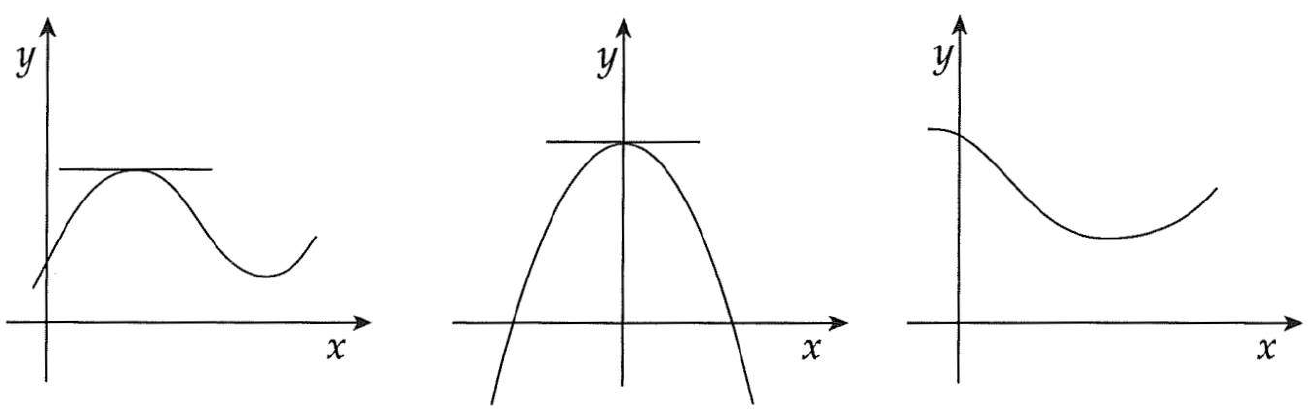
\includegraphics[scale=0.3]{images/figure_09_02.png} \end{figure}

Notice that, in all cases, $x*\geq0$, the derivative og the function at the point is either negative or is negative or zero, and the product of $x^*(df/dx)(x^*)$ is always zero. From here, we can conclude that the solution of the maximization problem  subject to the condition of non-negativity has to satisfy: $df/dx(x^*)\leq0$, $x^*\geq0$, and $x^*(df/dx)(x^*)=0$. The last condition, $x^*(df/dx)(x^*)$, is called the complementary condition.

This result can be generalized for problems with $n$ decision variables. For each variable, the partial derivative with respect to the variable has to be negative or zero; the value of the variable has to be non-negativity, and the product of the variable by the partial derivative has to be zero. To show this, we can make use of Taylor's formula:
$$f(\textbf{x}^*+t\textbf{u})-f(\textbf{x}^*)=t\nabla f(\textbf{x}^*)\cdot\textbf{u}+\frac{1}{2}t^2\textbf{u}'H(\textbf{x}^*+\theta t\textbf{u})\textbf{u},\ \theta\in(0,1)$$
As before, in order for $\textbf{x}^*$ to be a point where the function has a maximum, there will have to be a neighborhood $V(\textbf{x}^*)$ such that $f(\textbf{x}^*+t\textbf{u})-f(\textbf{x}^*)\leq0$ for all points that belong to that neighborhood and to the set of possibilities, $\forall(\textbf{x}^*+t\textbf{u})-f(\textbf{x}^*)\in V(\textbf{x}^*)\cap\{\textbf{x}\geq0\}$. 

If the point $\textbf{x}^*>0$, which means that all the decision variables are strictly positives, the vector $\textbf{u}$ any values, that is, we can move along in whichever direction (as long as $t$ is sufficiently small), without violating any of the non-negativity constraints. In this case, the necessary conditions for the existence of a local maximum are exactly equal to those studied before.

However, if any element of vector $\textbf{x}^*$ is zero, $x_j^*=0$, then the $j$ component of $\textbf{u}$ won't be able to be negative because $x_j$ cannot be negative. In this case, we won't also consider negative values of $t$, and for this reason, will just consider the case where $t\geq0$. We then conclude that: 
$$\lim_{t\to0}\left[\nabla f(\textbf{x}^*)\cdot\textbf{u}+\frac{1}{2}t\textbf{u}'H(\textbf{x}^*+\theta t\textbf{u})\textbf{u}\right]=0$$

In conclusion, the necessary conditions of first order are:
$$
\begin{cases}
	\frac{\partial f}{\partial x_i}(\textbf{x}^*)\leq0,\text{ for }i=1,\ 2,\dots,\ n;\\
	x^*_i\geq0,\text{ for }i=1,\ 2,\dots,\ n;\\
	x^*_i\frac{df}{dx_i}(\textbf{x}^*)=0,\text{ for }i=1,\ 2,\dots,\ n;\\
\end{cases}
$$
It is easy to show that for a problem of minimization subject to non-negativity constraints, the conditions are $\partial f/\partial x_i (\textbf{x}^*)\geq0$, $x^*_i\geq0$, and $x^*_i df/dx_i(\textbf{x}^*)=0$.

\addcontentsline{toc}{subsubsection}{9.2.2 Inequality constraints}
\subsubsection*{9.2.2 Inequality constraints}

The idea to address this type of constraints is to transform an inequality into equality. This happens with the introduction of a slack.

Consider the constraint $g_j(\textbf{x})\leq b_j$. The associated slack variable is $s_j=b_j-g_j(\textbf{x})$ (notice that $s_j>0$). The original constraint can therefor be rewritten as: $g_j(\textbf{x})+s_j=b_j$ and $s_j>0$. The optimization problem is then:
\begin{equation*}
\begin{aligned}
& \underset{\textbf{x},\textbf{s}}{\text{max}}
& & f(\textbf{x}) \\
& \text{s.t.}
& & g_1(\textbf{x})+s_1= b_1\\
& & & g_2(\textbf{x})+s_2= b_2\\
& & & \vdots\\
& & & g_m(\textbf{x})+s_m= b_m\\
& & & \textbf{x},\textbf{s}\geq0.
\end{aligned}
\end{equation*}

Now we have an optimization problem with equality and non-negativity constraints. By merging the Lagrangian with the non-negativity conditions from before, we get:
$$\Lagr(x_1,\dots,x_n,s_1,\dot,s_m,\lambda_1,\dots,\lambda_m)=f(x_1,x_2,\dots,x_n)+\sum_{j=1}^m\lambda_j(b_j-g_j(\textbf{x})-s_j).$$

The new first order conditions are:
\[
\left\{
\begin{aligned}
& \frac{\partial \Lagr}{\partial x_i} =\frac{\partial f}{\partial x_i}-\sum_{j=1}^{m}\lambda_j\frac{\partial g_j}{\partial x_i}\leq0 &\quad x_i\geq0 &\quad x_i\frac{\partial\Lagr}{\partial x_i}=0 &\quad i=1,\dots,n\\
& \frac{\partial \Lagr}{\partial s_j} =-\lambda_j\leq0 &\quad s_j\geq0 &\quad s_j\frac{\partial\Lagr}{\partial s_j}=0 &\quad j=1,\dots,m \\
& \frac{\partial \Lagr}{\partial \lambda_j} =b_j-g_j(\textbf{x})-s_j=0 & & & j=1,\dots,m.
\end{aligned}\right.
\] 

Let us analyze the second set of constraints. The first constraint says that $\partial\Lagr/\partial s_j=-\lambda_j\leq0$, and from here we can conclude that $\lambda_j\geq0$. The second condition says that $s_j\geq0$, but as $s_j=b_j-g_j(\textbf{x})$, this is equivalent to saying that the $b_j-g_j(\textbf{x})\geq0$, which means that the constraint $j$ has to be satisfied. Finally, $s_j\partial\Lagr/\partial s_j=0$ which is equivalent to $\lambda_j(b_j-g_j(\textbf{x}))=0$.

While it would be possible to solve an optimization problem with inequality constraints via the slack method, it is not common. Why? The conditions above are equivalent to those of the problem of finding a saddle point with the Lagrangian without the inclusion of the slack variables. That is, we would want to find the values of $\textbf{x}^*$ and $\boldsymbol{\lambda}^*$ such that the Lagrangian function has a maximum at $\textbf{x}^*$ and a minimum at $\boldsymbol{\lambda}^*$. The Lagrangian function is then:
$$\Lagr(\textbf{x},\boldsymbol{\lambda})=f(\textbf{x})+\sum_{j=1}^{m}\lambda_j(b_j-g_j(\textbf{x})).$$
And the first order conditions if this problem are:
\[
\left\{
\begin{aligned}
& \frac{\partial \Lagr}{\partial x_i} =\frac{\partial f}{\partial x_i}-\sum_{j=1}^{m}\lambda_j\frac{\partial g_j}{\partial x_i}\leq0 \quad &\quad x_i\geq0 \quad&\quad x_i\frac{\partial\Lagr}{\partial x_i}=0 \quad &\quad i=1,\dots,n\\
& \frac{\partial \Lagr}{\partial \lambda_j} =b_j-g_j(\textbf{x})\geq0 \quad&\quad \lambda_j\geq0 \quad&\quad\lambda_j\frac{\partial\Lagr}{\partial \lambda_j}=0   \quad&\quad j=1,\dots,m.
\end{aligned}\right.
\] 

We can verify that these conditions are in fact equivalent to the conditions with the slacks. These new conditions are called Kuhn-Tucker conditions. Notice that, while the sign of the partial derivative of the Lagrangian with regards to the decision variable is not positive ($\leq0$), the sign of the partial derivatives with regards to the Lagrangian multipliers is non-negative ($\geq0$). This should not come as a surprise as it results of the fact that we want a maximum at $\textbf{x}$ and a minimum at $\boldsymbol{\lambda}$, and that in a problem of minimization with non-negativity constraints, the partial derivatives have to be bigger or equal to zero.

The same way as before, $\partial\Lagr/\partial\lambda_j\geq0$ tells us that the constraint $j$ has to be satisfied (in practical terms, this implies that one needs not to memorize the sign of the derivative $\partial\Lagr/\partial\lambda_j$, as it can be deduced from the constraint).

Once again, if we have a minimization problem, and the decision variable $x_i$ has to be non-negative, $\partial\Lagr/\partial x_i$ has to be bigger or equal to zero, simultaneously verifying the constraints of non-negativity, $x_i\geq0$, and complementarity, $(\partial\Lagr/\partial x_i)x_i=0$.

If the decision variable $x_i$ can take any value, $\partial\Lagr/\partial x_i$ will have to be equal to zero, regardless if the problem is a maximization or minimization.

The sign of $\partial\Lagr/\partial\lambda_j$ only depends on the type of constraint, as $\partial\Lagr/\lambda_j$ only tells us if the constraint is satisfied. As $\partial\Lagr/\partial\lambda_j=b_j-g_j(\textbf{x})$, it is immediate that, if the constraint is $g_j(\textbf{x})\leq b_j$,  $\partial\Lagr/\lambda_j$ is bigger or equal to zero. On the other hand, if the constraint is $g_j(\textbf{x})\geq b_j$,  $\partial\Lagr/\lambda_j$ is lower or equal to zero.

The only aspect that is not immediate is the sign of the multiplier.

\addcontentsline{toc}{subsubsection}{9.2.3 The signs of the Lagrangian multipliers}
\subsubsection*{9.2.3 The signs of the Lagrangian multipliers}

Previously, we showed that the Lagrangian multiplier associated to a given constraint, $j$, tells us what is the variation on the optimal value of the function when the constant $b_j$ increases. The most intuitive way of studying the multipliers is to: first, what happens to the optimal value of the objective function when the opportunity set expands or contracts; and, after, how does the opportunities set changes when $b_j$ increases.

It is clear that, if the opportunities set increases and we are maximizing, then value of the objective function can never decrease as we still have all possible points from before plus new points that may or not increase the function. If worse, we may always keep using the previous better point. On the other hand, if the set decreases, then the value may or not decrease depending on whether the old point is still possible or not. With this, we can understand the sign of the Lagrangian multipliers.

Consider the inequality constraint $g_j(\textbf{x})\leq b_j$. An increase of $b_j$ corresponds to an enlargement of the opportunities set. This implies that if we are 
maximizing, the value of the objective function either stays the same or increases, that is, $\lambda\geq0$. On the other hand, if we are minimizing, the value of the objective function either stays the same or goes down, that is, $\lambda\leq0$.

\addcontentsline{toc}{subsubsection}{9.2.4 Conditions of complementarity}
\subsubsection*{9.2.4 Conditions of complementarity}

In the case of the decision variables, the complementarity conditions $x_i\frac{\Lagr}{\partial x_i}=0$ tell us that, at the optimal, either the variable is zero, or the partial derivative of the Lagrangian function with respect to the variable is zero, or both. There are a couple of thing we can conclude from here:
\begin{itemize}
	\item If, at the optimal, the variable is positive, $x_i>0$, then the partial derivative of the Lagrangian function with respect to the variable is zero, $\partial\Lagr/\partial x_i=0$;
	\item If, at the optimal, the partial derivative of the Lagrangian function with respect to the variable is negative, $\partial\Lagr/\partial x_i<00$, then the variable must be zero, $x_i=0$.
\end{itemize}

In the case of the Lagrangian multipliers, the complementarity condition can be written as $\lambda_j(b_j-g_j(\textbf{x}))=0$, which tells us that the constraint is satisfied as an equality, the shadow price associated to the constraint is zero, or both. When, at the optimal, the constraint is satisfied as an equality, it all tells us that the constraint is binding. There are a couple of things that we can conclude from the the complementarity conditions:
\begin{itemize}
	\item If, at the optimal, the shadow price is positive, $\lambda_j>0$, then the corresponding constraint has to be binding, $g_j(\textbf{x})=b_j$;
	\item If, at the optimal, the constraint is not binding, that is $g_j(\textbf{x})<b_j$, then the corresponding multiplier is zero. The rational is that, given that we are no using a certain resource as much as we could, we do not value having more of that resource, as its shadow price is zero.
\end{itemize}

\addcontentsline{toc}{subsection}{9.3 Discussion on the Kuhn-Tucker conditions}
\subsection*{9.3 Discussion on the Kuhn-Tucker conditions}

Writing the Kuhn-Tucker conditions is an easy task once understood the intuition behind the signs of the multipliers and of $\partial\Lagr/\partial\textbf{x}$. However, verifying if a point, $(\textbf{x}^*, \boldsymbol{\lambda}^*)$, satisfies the Kuhn-Tucker conditions is not, in general, that easy. The problem is that we have to solve a system of equations. What to do, then?

The usual first step is to study the different possible cases, that is, which are the decision variables and multipliers that are different from zero and which are equal to zero. We then have a system of equations made up of equations of derivatives that are zero, and by equations that respect the null variables.

If this system does not have a solution, we can immediately conclude that the hypothesis considered does not solve the system of inequalities. If the system has a solution, then we have to verify that, for the values that satisfy it, all other Kuhn-Tucker conditions are met. If they are, our solution satisfies the Kuhn-Tucker conditions, and, for this reason, we do not need to move to a new hypothesis which can continuously happen until we exhaust all hypothesis. 

\addcontentsline{toc}{subsection}{9.4 Kuhn-Tucker theorem}
\subsection*{9.4 Kuhn-Tucker theorem}

\addcontentsline{toc}{subsubsection}{9.4.1 Sufficiency theorem}
\subsubsection*{9.4.1 Sufficiency theorem}


$\textbf{Theorem 9.1}$ If a function $f$ is concave and differentiable on the non-negative quadrant, if the constraints $g_j$ are convex and differentiable on the non-negative quadrant, and if $(\textbf{x}^*,\boldsymbol{\lambda}^*)$ satisfies the Kuhn-Tucker conditions, then $f(\textbf{x}^*)$ is the global maximum of the problem:
$$\max_\textbf{x}f(\textbf{x})\text{ s.t. }\textbf{g}(\textbf{x})\leq\textbf{b},\ \textbf{x}\geq0.$$
\noindent\rule{\textwidth}{1pt}

This theorem tells us the conditions that guarantee tha $\textbf{x}^*$ is a solution fo the maximization problem. That is, these conditions are sufficient for $f(\textbf{x}^*)$ to be a global maximum of the problem. However, under which conditions can we guarantee that the $f(\textbf{x}^*)$ is a strict global maximum? If the objective function is strictly concave then the global maximum is strict.

We now could as: what are the circumstances in which the Kuhn-Tucker conditions are necessary for the existence of an optimal point?

\noindent\rule{\textwidth}{1pt}

$\textbf{Theorem 9.2}$ Under certain conditions, $\textbf{x}^*$ is solution of the optimization problem:
$$\max_\textbf{x}f(\textbf{x})\text{ s.t. }\textbf{g}(\textbf{x})\leq\textbf{b},\ \textbf{x}\geq0.$$
if there is at least a vector $\boldsymbol{\lambda}^*$ such that $(\textbf{x}^*,\boldsymbol{\lambda}^*)$ is a solution of the saddle point problem, that is, that it satisfies the Kuhn-Tucker conditions.


\addcontentsline{toc}{subsubsection}{9.4.2 Restriction of qualification}
\subsubsection*{9.4.2 Restriction of qualification}

$\textbf{Theorem 9.3}$ If any of the following conditions is satisfied, then the qualification constraint is satisfied and, therefor, the Kuhn-Tucker conditions are necessary:
\begin{itemize}
	\item The $g_j$ functions are linear;
	\item The $g_j$ functions are convex, and there is a point $\textbf{x}\in X$ such that $g_i\leq b_j$, for all the linear constraints, and $g_i< b_j$ for the non-linear constraints;
	\item The set of opportunities is convex, with a non-empty interior, and, whichever the boundary point $\overline{\textbf{x}}$, $\nabla g_j\neq0$ for all binding constraints at $\overline{\textbf{x}}$;
	\item Whichever the boundary point $\overline{\textbf{x}}$, the characteristic of the jacobian matrix of the binding constraints, $\left[\partial\textbf{g}/\partial\textbf{x}\right]_{\overline{\textbf{x}}}$, is equal to the number of binding constraints at that point.
\end{itemize}

\noindent\rule{\textwidth}{1pt}

Notice that it is enough for one of the above conditions to be met for the Kuhn-Tucker conditions to be necessarily verifies at the optimizing point.

While this may seem restrictive, the first condition is met in most economic problems. For example, the first condition is find in all problems of linear programming, as long as the constraints and objective function are linear.

The second condition implies that, when the interior points of the opportunities set is non-empty, and the functions $g_j$ are all convex, the Kuhn-Tucker conditions are necessary. As it is relatively easy to verify the convexity of functions, and that the interior of $X$ is non-empty, this condition is quite useful.

With regards to the third condition, it is worth remembering what makes an opportunities set to be convex. If the constraints of type $g_j(\textbf{x})\leq b_j$, and the function $g_j(\textbf{x})$ is quasi-convex, then the set of points that satisfies the constraint is a convex set.

Curiously, the forth condition is the same as the one we applied in the case of an optimization with equality constraints. Previously, we saw that, in order to apply the method of the Lagrangian multipliers, the characteristic of the jacobian matrix of $\textbf{g}$ has to be equal to the number of restrictions, $m$. However, in that type of problems, all constraints have to be satisfied as an equality, that is, all constraints are binding.

Notice that in the last two conditions all the points of the boundary have to be verified, as the binding restrictions depend on which boundary point is being considered.

\addcontentsline{toc}{subsection}{9.5 Quasi-concave programming}
\subsection*{9.5 Quasi-concave programming}

Quasi-concave functions are of particular interest as they satisfy an extra couple of conditions that make the Kuhn-Tucker conditions both necessary and sufficient.

$\textbf{Theorem 9.4}$ Consider $f$ and $g_1,\ g_2,\dots,\ g_m$ real functions of real variables, differentiable, with $f$ quasi-concave, and $g_1,\ g_2,\dots,\ g_m$ quasi-convex. Then, if $(\textbf{x}^*,\boldsymbol{\lambda}^*)$ is a solution of the saddle point, then $\textbf{x}^*$ is also a solution of the problem:
$$\max_\textbf{x}f(\textbf{x})\text{ s.t. }\textbf{g}(\textbf{x})\leq\textbf{b},\ \textbf{x}\geq0,$$
as long as one of the following conditions is verified:
\begin{itemize}
	\item $\left(\frac{\partial f}{\partial x_i}\right)_{\textbf{x}^*}<0$ for at least one of the variables;
	\item $\left(\frac{\partial f}{\partial x_i}\right)_{\textbf{x}^*}>0$ for at least one of the variables, such that $x^*_j>0$;
	\item $\nabla f(\textbf{x}^*)\neq\textbf{0}$, and the function $f$ is of class $C^2$;
	\item The function $f$ is concave.
\end{itemize}

While this is certainly going overboard, it is important to remember that there are certain conditions in which, if the objective function is quasi-concave, and the functions $g$ are quasi-convex, the Kuhn-Tucker conditions for the maximization problem subject to conditions of the $\leq$ type are necessary and sufficient.

\vspace*{\fill} 
\begin{quote} 
	\centering 
	\textit{``Viva o Xufrimento!''} 
\end{quote}
\vspace*{\fill}

\end{document}  